
\subsection{$\PH \to \ZZ \to 2\ell 2\ell '$}

This analysis seeks to identify Higgs boson decays to a pair of $\cPZ$ bosons, with both decaying to a pair of
leptons (electron, muon or tau). This channel has extremely low background, and the presence of four leptons in the
final state allows reconstruction and isolation requirements to be very loose. Due to high efficiency of the 
selection requirements, this channel is one of the major discovery channels at both low and high Higgs boson masses.
A detailed description of this analysis may be found in~\cite{CMSobservation125,Chatrchyan:2012dg,Chatrchyan:2012hr}.

Events included in the analysis contain $\cPZ$ candidates formed from a pair of leptons of the same flavor and
opposite charge. Decay electrons and muons are required to be isolated, and to originate from the primary vertex.
Electrons (muons) are required to have $\pt > 7(5)\GeV$ and $|\eta|<2.5(2.1)$, and taus are required to have
$\PT > 20 \GeV$ and $|\eta|<2.3$. The event selection procedure results in mutually-exclusive sets of Z candidates
in the $\PH\rightarrow 2\ell 2\ell$ and $\PH\rightarrow 2\ell2\Pgt$ channels, with the former identified first.

For the $2\ell2\ell$ final state, the lepton pair with invariant mass closest to the nominal $\cPZ$ mass, denoted
$\cPZ_1$, is identified and retained if it satisfies $40 < m_{\cPZ_1} < 120\GeV$. The second $\cPZ$ is then
constructed from the remaining leptons in the event, and is required to satisfy $12 < m_{\cPZ_2} < 120\GeV$. If
more than one $\cPZ_2$ candidate remains, the ambiguity is resolved by choosing the leptons of highest $\pt$. Amongst
the four candidate decay leptons, it is required that at least one should have $\PT > 20\GeV$, and that another
should have $\PT > 10\GeV$. This requirement ensures that selected events correspond to the high-efficiency
plateau of the trigger.

%% ED: The statement on the ambiguity is itself amiguous. Does it mean 'the candidate containing the remaining lepton of highest pt', or 'the candidate with the highest pt_z', or something else?

For the $2\ell2\Pgt$ final state, events are required to have one $\cPZ_1 \to \ell^+\ell^-$ candidate, with one
lepton having $\PT > 20\GeV$ and the other $\PT > 10\GeV$, and a $\cPZ_2 \to \Pgt^+\Pgt^-$, with $\Pgt$ decaying
via $\Pgm, \Pe$ or hadrons. The leptons from $\Pgt$ leptonic decays are required to have $\PT > 10\GeV$. The invariant
mass of the reconstructed $\cPZ_1$ is required to satisfy $60 < m_{\ell\ell} < 120\GeV$, and that of the $\cPZ_2$ to
satisfy $ m_{\Pgt\Pgt} < 90\GeV$, where $m_{\Pgt\Pgt}$ is the invariant mass of the visible tau decay products.

Simulation is used to evaluate the local density of events expected as a function of $m_{2\ell2\ell'}$ from the
$\cPZ\cPZ$ background, $\Delta N / \Delta m_{2\ell2\ell'}$. The cross section for \ZZ\ production at NLO is
calculated with \textsc{mcfm}~\cite{MCFM,Campbell:1999ah,Campbell:2011bn}. The theoretical uncertainty on the
cross-section is evaluated as a function of $m_{2\ell2\ell'}$, varying both the QCD renormalisation and factorization
scales and the PDF set, following the PDF4LHC recommendations~\cite{Botje:2011sn,Alekhin:2011sk,Lai:2010vv,Martin:2009iq,Ball:2011mu}. The uncertainty associated
with the QCD and PDF scales for each final state are on averages 8\%. The number of predicted $\ZZ \to 2\ell 2\ell'$
events, and their associated uncertainties, after the signal selection are given in Table~\ref{tab:SelectYields}.

%% ED: Should the reference to MCFM go into section 2, along with the other simulation details?

To allow estimation of the $\ttbar$, $\cPZ$+jets, and $\PW\cPZ$+jets backgrounds, a $\cPZ_1$+X control region 
is
defined, 
%in the Higgs boson mass distribution, 
well separated from the expected signal region.
% for each mass hypothesis.
In addition, a sample of $\cPZ_1 + \ell_\text{reco}$ events, with at least 
one reconstructed lepton in addition to a $\cPZ$, is
defined in order to estimate the lepton misidentification probability, the probability for a fake lepton to be reconstructed and pass the isolation and identification requirements. The contamination of the sample from $\PW\cPZ$ events containing a
real additional lepton is suppressed by requiring the imbalance of the measured energy deposition in the transverse
plane to be below $25\GeV$. The event rates measured in the background control region are extrapolated to the
signal region, and are presented in Table~\ref{tab:SelectYields}. The systematic uncertainties associated with the 
reducible background estimate vary from 30\% to 100\%, and are presented in the table combined in quadrature with
the statistical uncertainties.

%% ED: The statement about the 'imbalance of measured energy deposition' is not clear. Does this refer to the whole event (ie just event MET) or to the Z and lepton candidate?

%% ED: The original text on the control region and lepton misidentification were not clear. Check that I have actually written what was done.

%% ED: 'squared' -> 'combined in quadrature' - hopefully this is what was meant.

%============
\begin{table}[htbp]
\begin{center}
\caption{
Event candidates observed, compared to the expected background and signal rates for each final state in the
$\PH \to \ZZ \to 2\ell 2\ell '$ channel. For the $\cPZ$+X background, the estimations are based on data.
The uncertainties represent the statistical and systematic uncertainties combined in quadrature.
}
\label{tab:SelectYields}
\begin{tabular}{l|c|c|c|c|c}
\hline
\textbf{Channel} & $4\Pe$ & $4\Pgm$ & $2\Pe2\Pgm$ & $4\ell$ & $2\ell2\Pgt$  \\
\hline
\cPZ\cPZ\ background &  29.3  $\pm$  3.4 &  49.0  $\pm$  5.1  &  75.5  $\pm$  8.0 &  153.7 $\pm$ 10.1 & 12.1 $\pm$ 1.5 \\ %
\cPZ+X                            &   $3.0 ^{ +  2.7 }_{ -  1.9 }$ &  $2.2 ^{ +  1.6 }_{ -  1.3 }$ &  $5.0 ^{ +  4.0 }_{ -  3.0 }$  & $10.2 ^{ +  5.0 }_{ -  3.8 }$ & 8.9  $\pm$ 2.5  \\ % 
\hline
All backgrounds    &   $32.3 ^{ +  4.4 }_{ -  3.9 }$ &  $51.2 ^{ +  5.3 }_{ -  5.3 }$ &  $80.5 ^{ +  9.0 }_{ -  8.6 }$ &  $163.9 ^{ +  11.3 }_{ -  10.8 }$ & 21.0 $\pm$ 2.9  \\ % 
%~~~($100 < m_{4\ell} < 130\GeV$)   &    X.XX $\pm$ XX  & X.XX $\pm$ XX &   X.XX $\pm$ XX  & --  \\ % 5/fb
\hline
Observed  & 32 & 47  & 93 & 172 & 20 \\ % 5/fb
\hline
$\mH = 200\GeV$ & 8.3  $\pm$  2.0  &  13.3  $\pm$  2.7  &  21.6  $\pm$  4.5 &  43.2  $\pm$ 5.6 &  2.9 $\pm$ 0.7  \\ % 
$\mH = 350\GeV$ & 4.8  $\pm$  1.2  &  7.5  $\pm$  1.6  &  12.7  $\pm$  2.9 &  24.9  $\pm$  3.5 &  3.1 $\pm$ 0.8 \\ % 
$\mH = 500\GeV$ & 1.7  $\pm$  0.8  &  2.6  $\pm$  1.2  &  4.4  $\pm$  2.0 &  8.7  $\pm$  2.4 &   1.4 $\pm$ 0.7 \\ % 
\hline
\end{tabular}
\end{center}
\end{table}

The reconstructed invariant mass distribution for $2\ell 2\ell$, combining the $4\Pe$, $4\Pgm$, and $2\Pe2\Pgm$
channels, is shown in Figure~\ref{fig:Mass4l-2l2tau}, compared with the expectation from SM background processes.
The figure also shows the reconstructed visible mass distributions for the $2\ell2\Pgt$ selection, combining all
the $2\ell2\tau$ final states. The background shapes are taken from simulation, with rates normalized to data.
The observed mass distributions are well-matched to the SM background expectation.

%=============
\begin{figure}[htbp]
\begin{center}
%
%{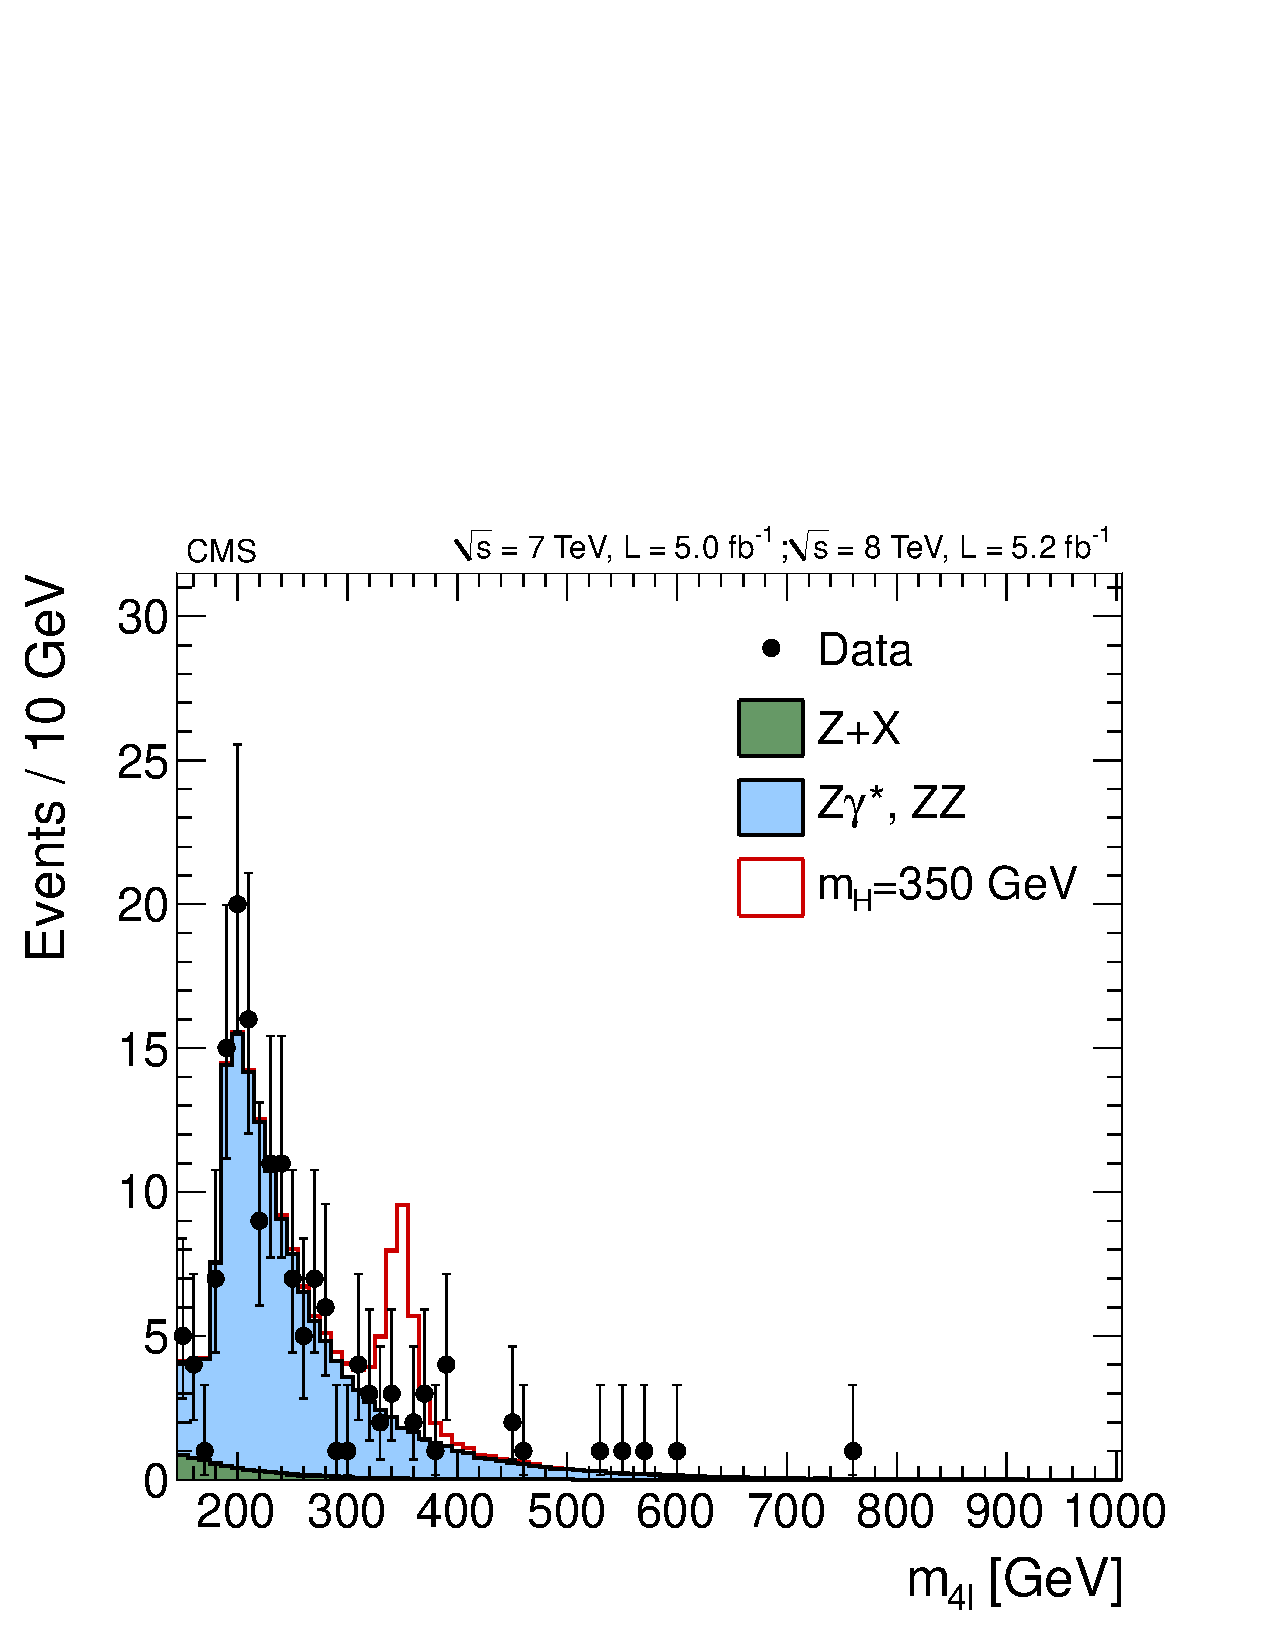
\includegraphics[width=0.44\textwidth]{plots/hzz4lmass.pdf}}
%{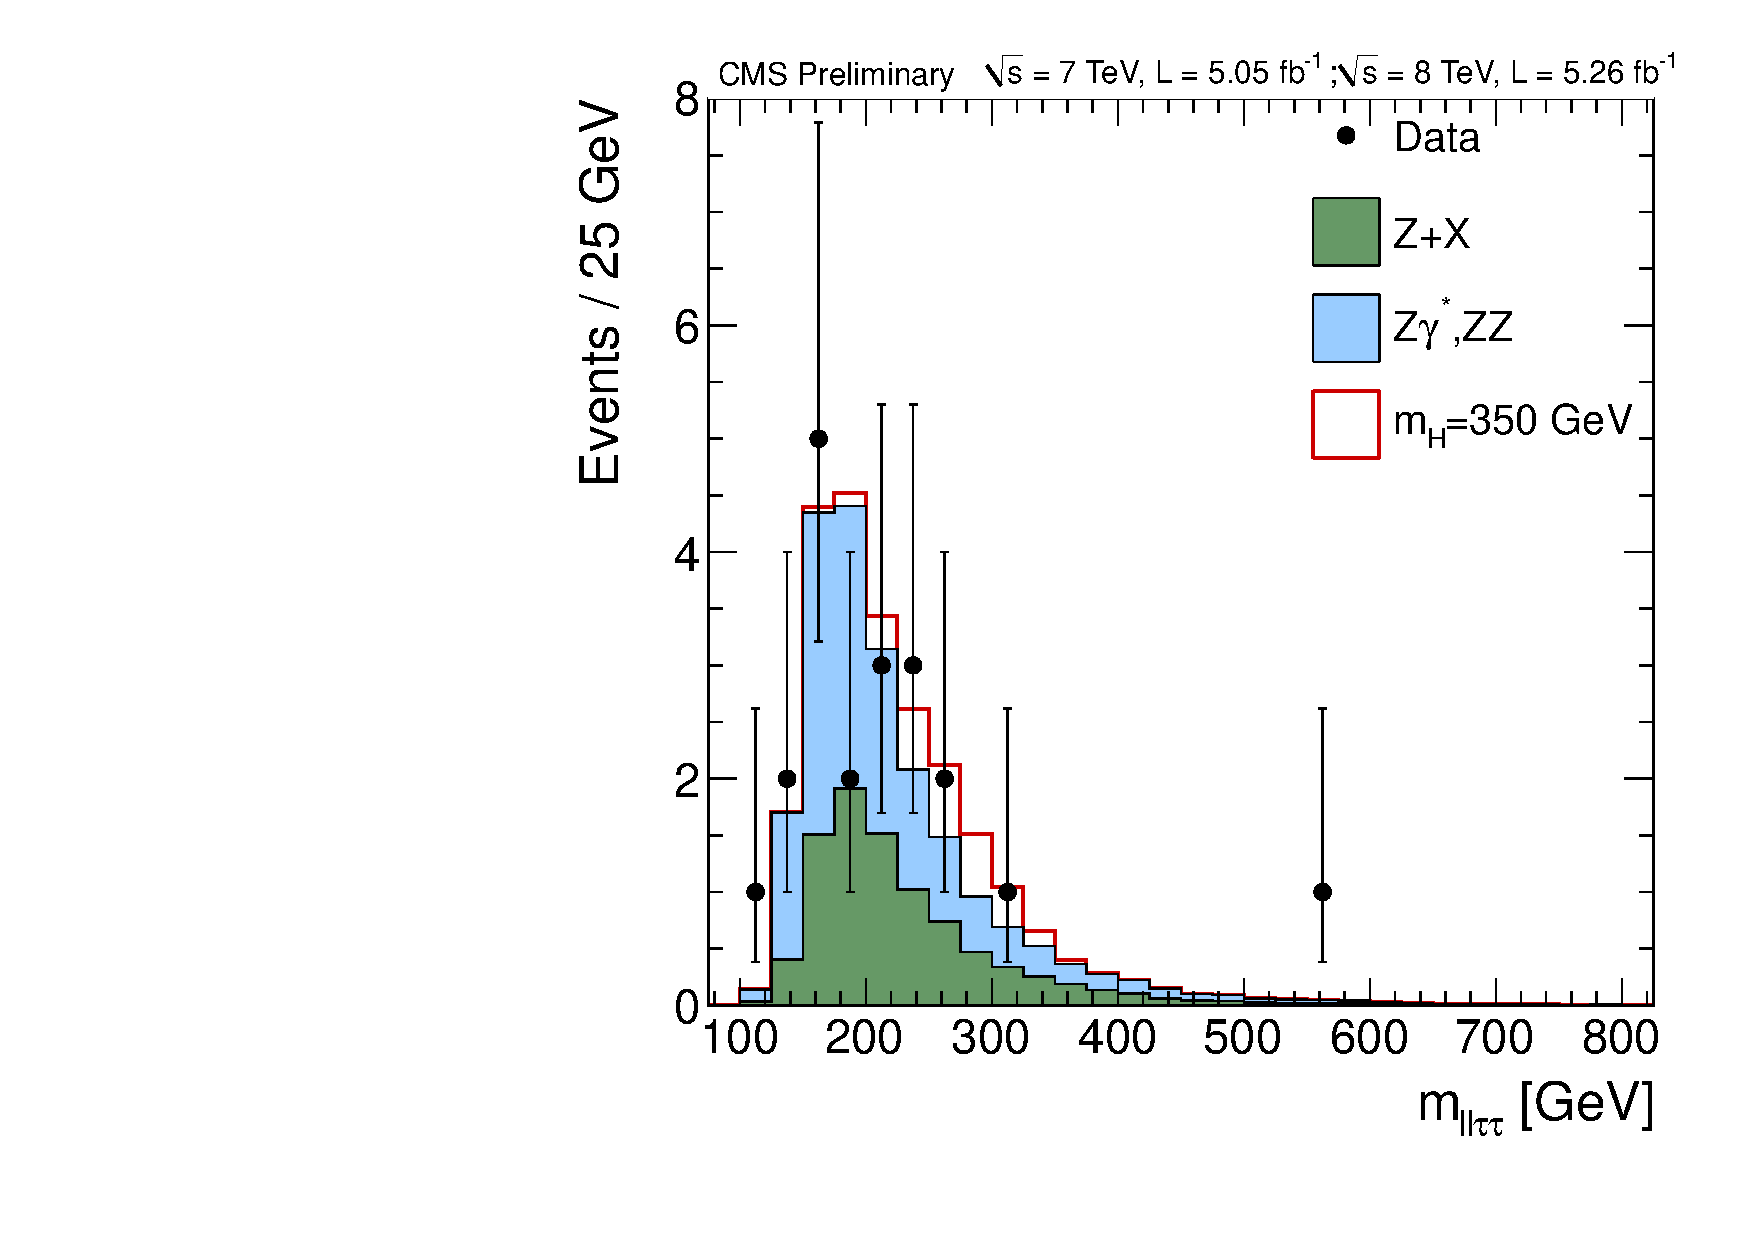
\includegraphics[width=0.4\textwidth]{plots/2l2taumass.pdf}}
\subfigure[]{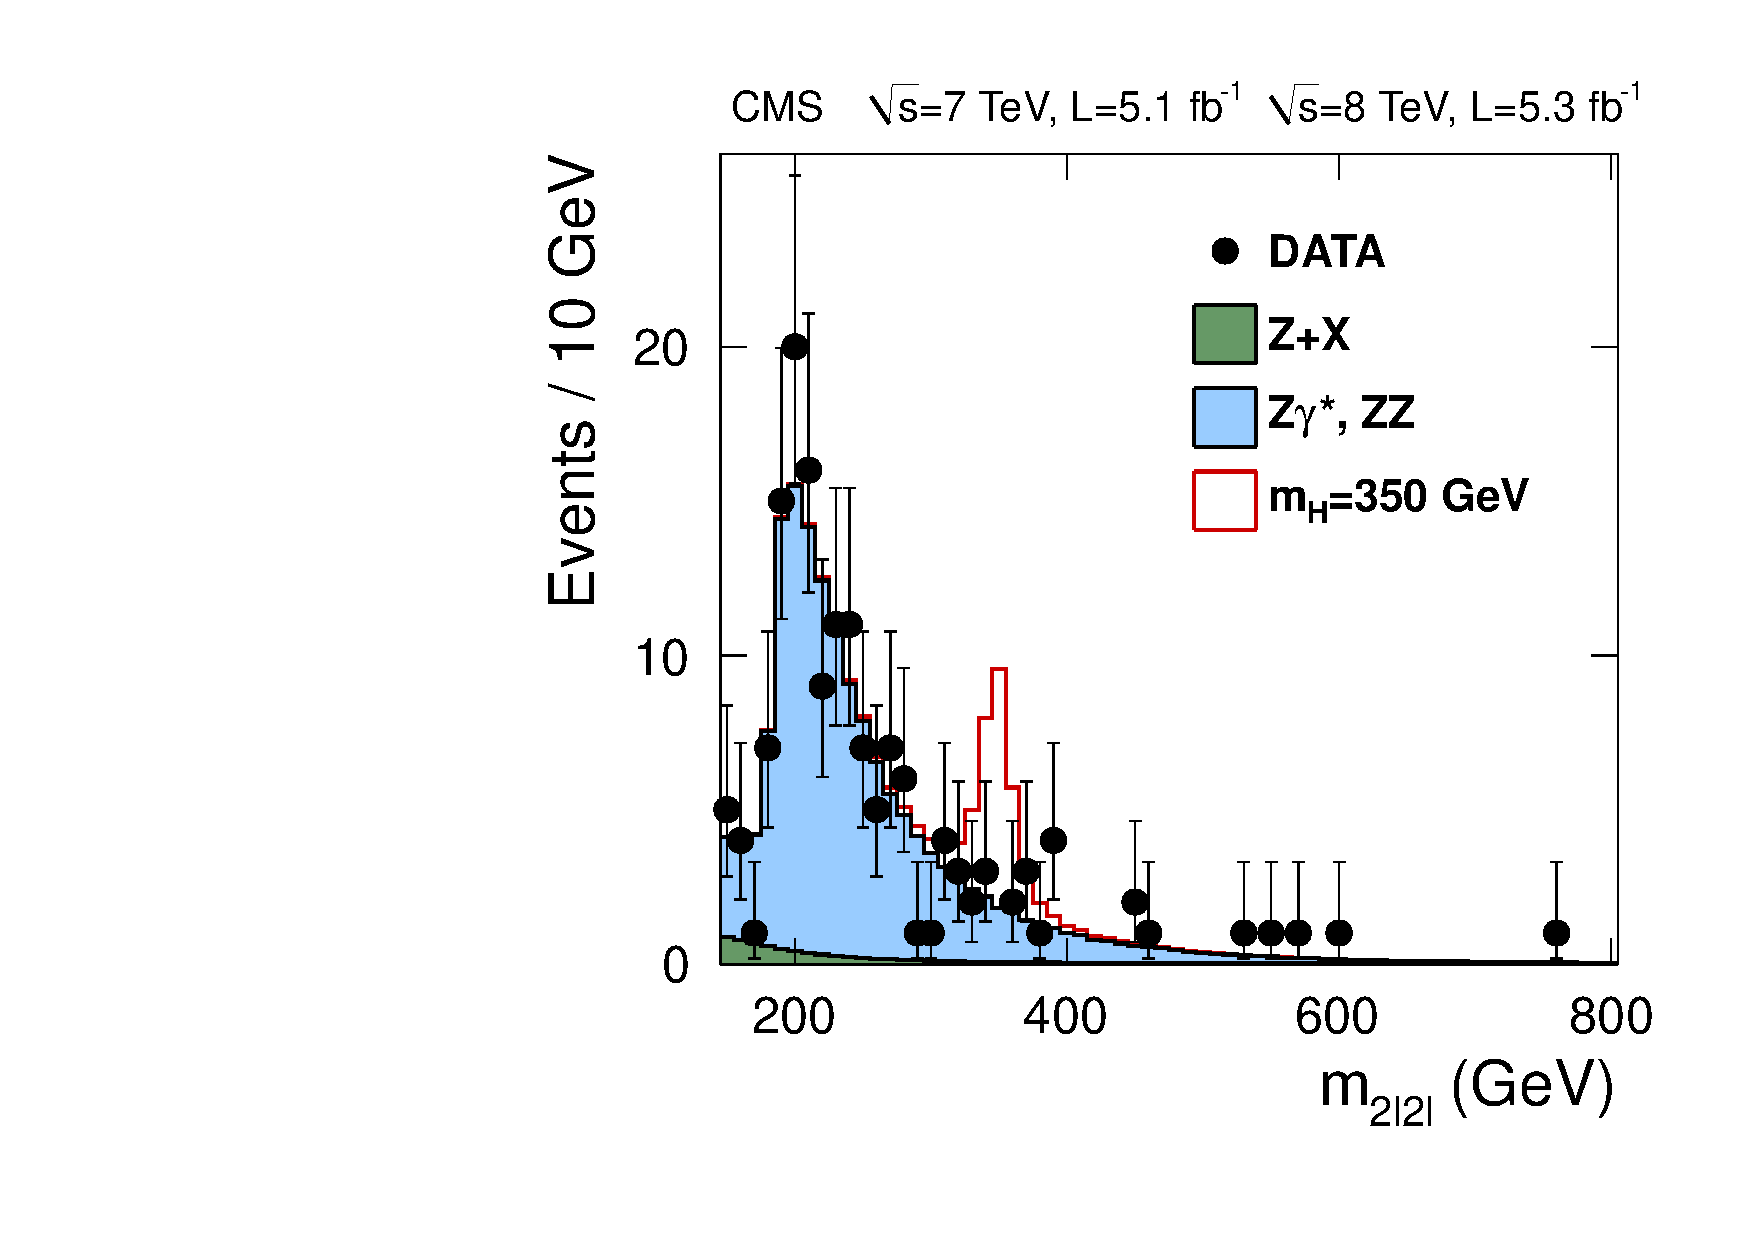
\includegraphics[width=0.45\textwidth]{figures/ZZ4lmass}}
\subfigure[]{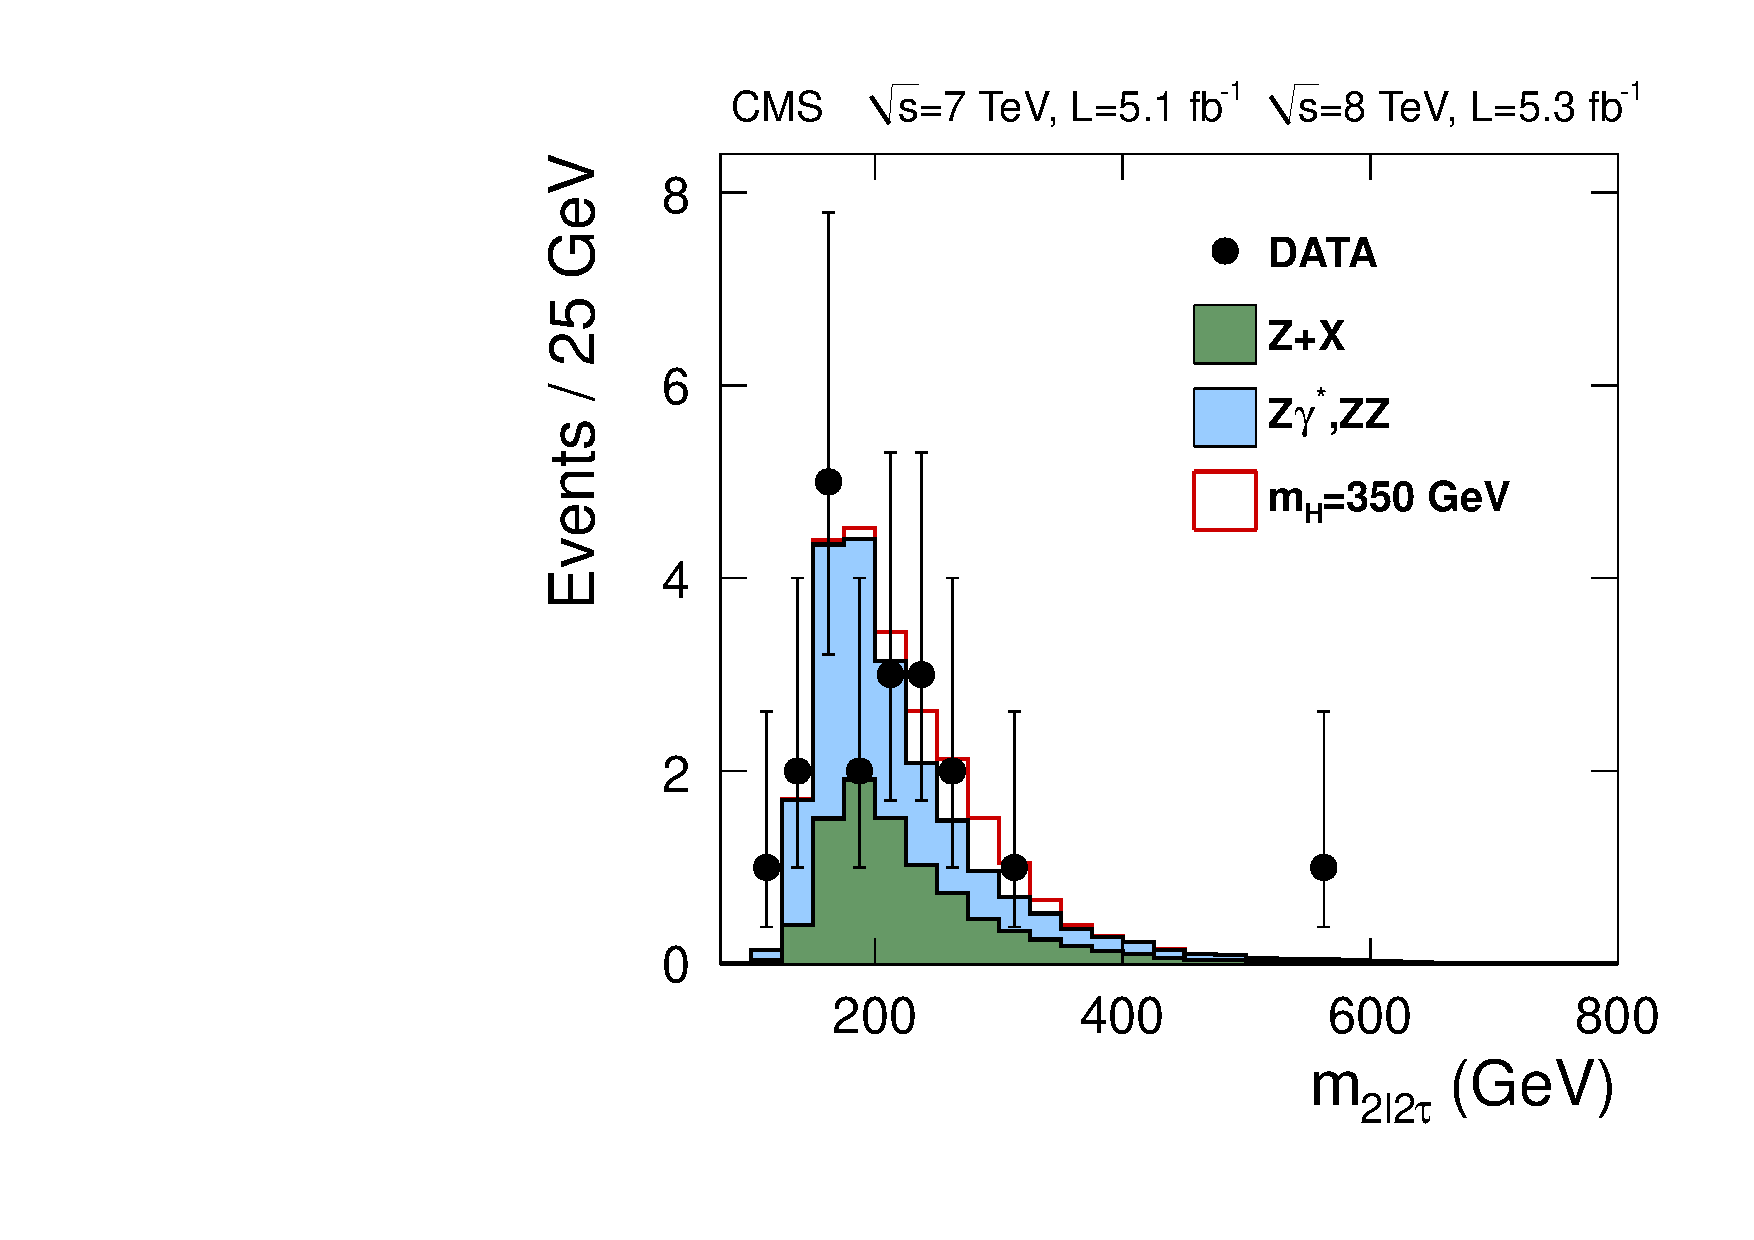
\includegraphics[width=0.45\textwidth]{figures/ZZ2l2tauMass.pdf}}
%
\caption{ 
Distribution of the four-lepton reconstructed mass for (a) the sum of 
the $4\Pe$, $4\Pgm$, and $2\Pe2\Pgm$ channels , and for (b) the sum over all
$2\ell2\tau$ channels.
Points represent the data, shaded histograms represent the background 
and unshaded histogram the signal expectations.
The distributions are presented as stacked histograms. 
The reconstructed masses in $2\ell2\tau$ states
are shifted downwards with respect to the true masses by about 
30\% due to the
undetected neutrinos in $\tau$ decays.
}
\label{fig:Mass4l-2l2tau}
\end{center}
\end{figure}
%=======

%
%=======
\begin{figure}[htbp]
\begin{center}
%
%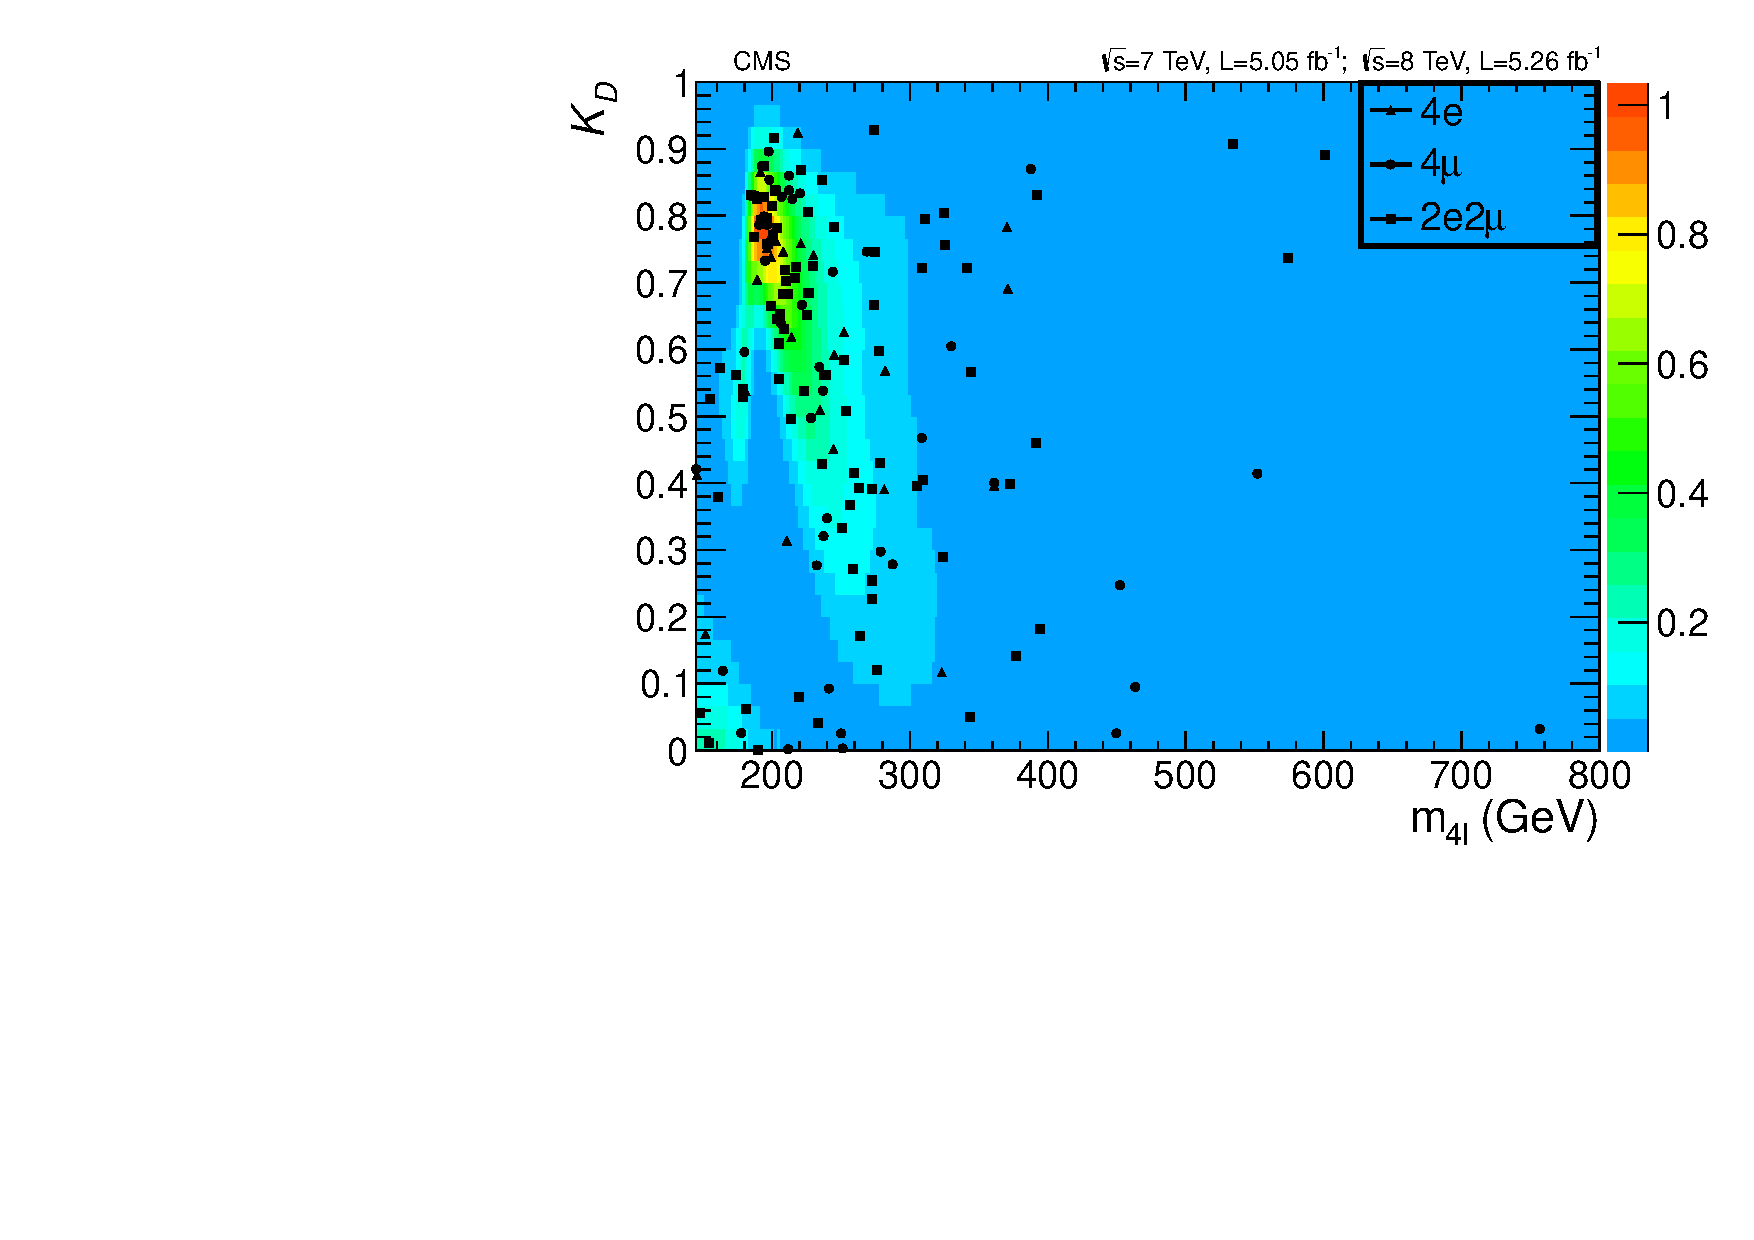
\includegraphics[width=0.5\linewidth]{plots/hzz4lmela.pdf}
%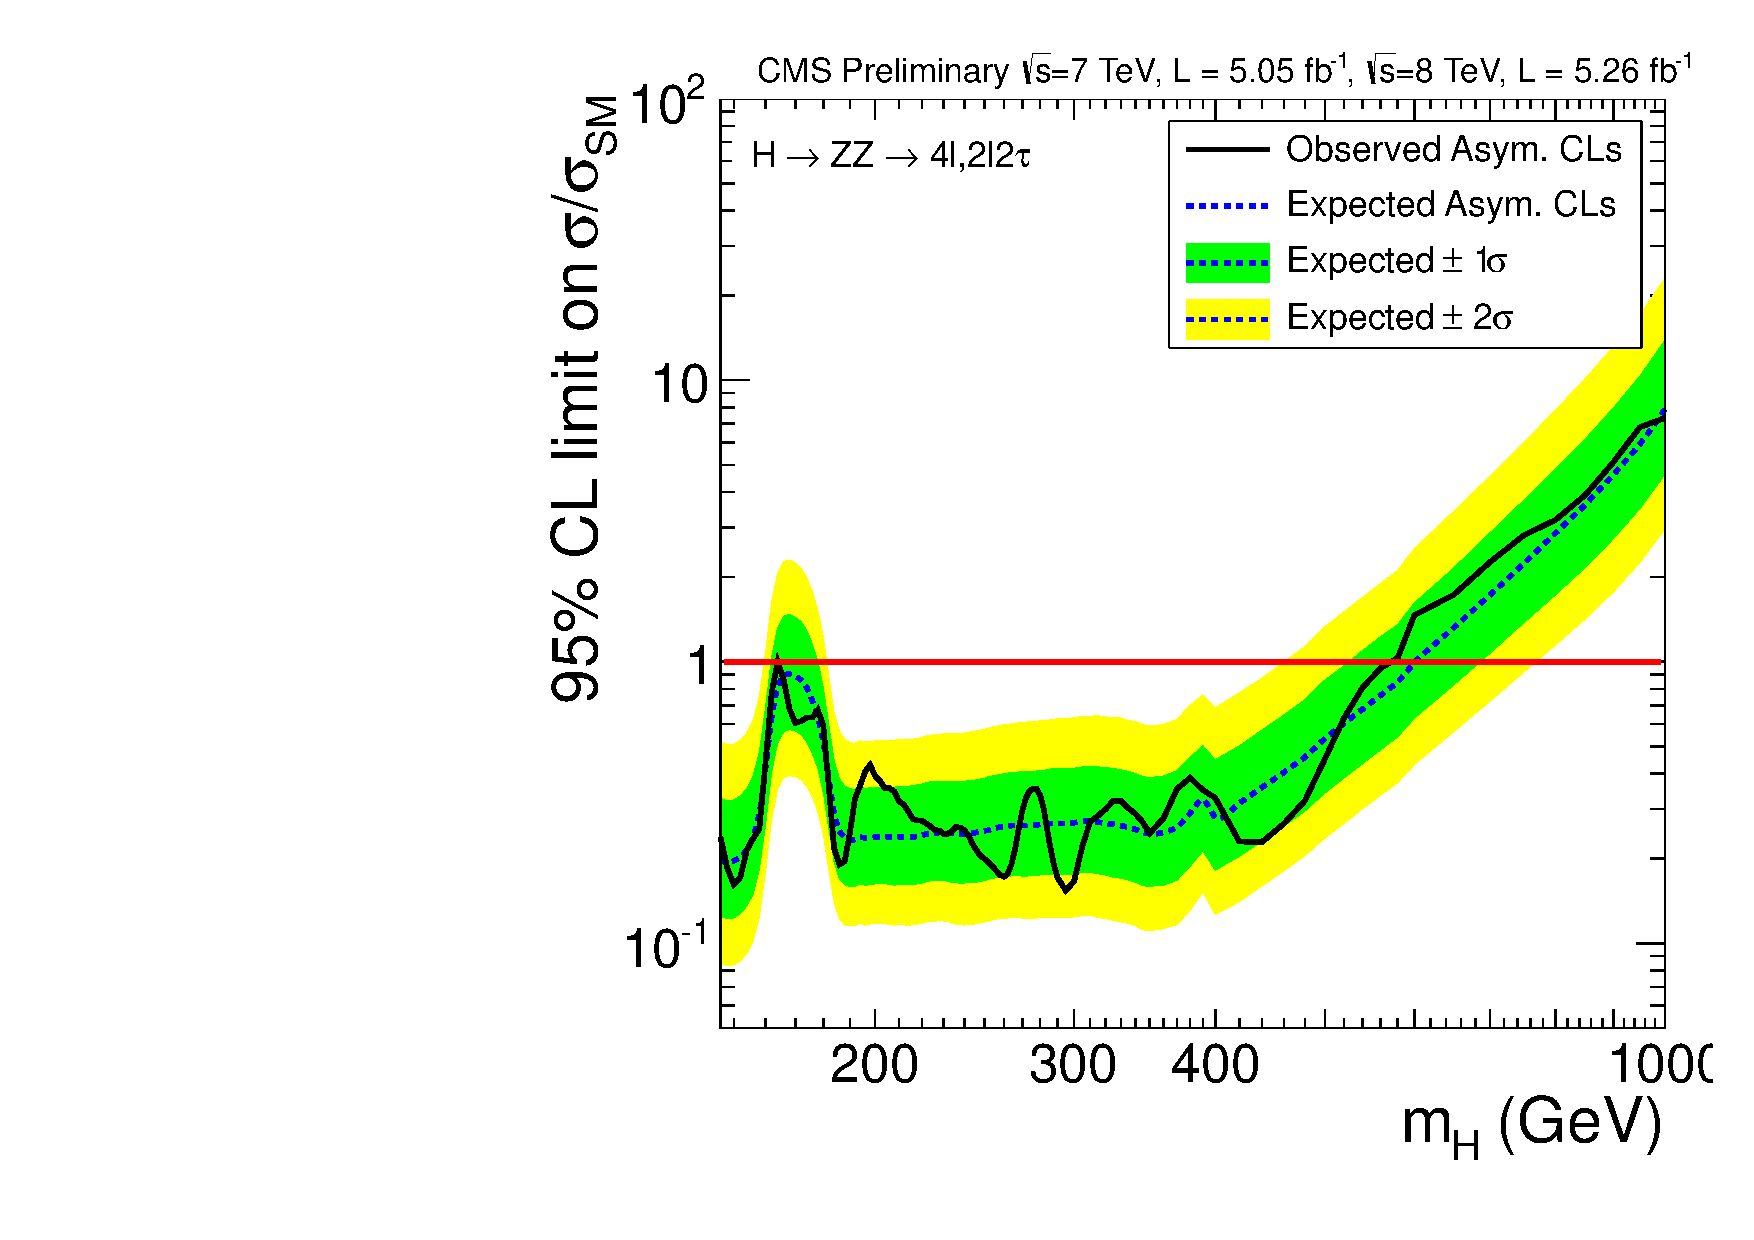
\includegraphics[width=0.4\linewidth]{plots/hzz4llimit7and8TeV.pdf}
\subfigure[]{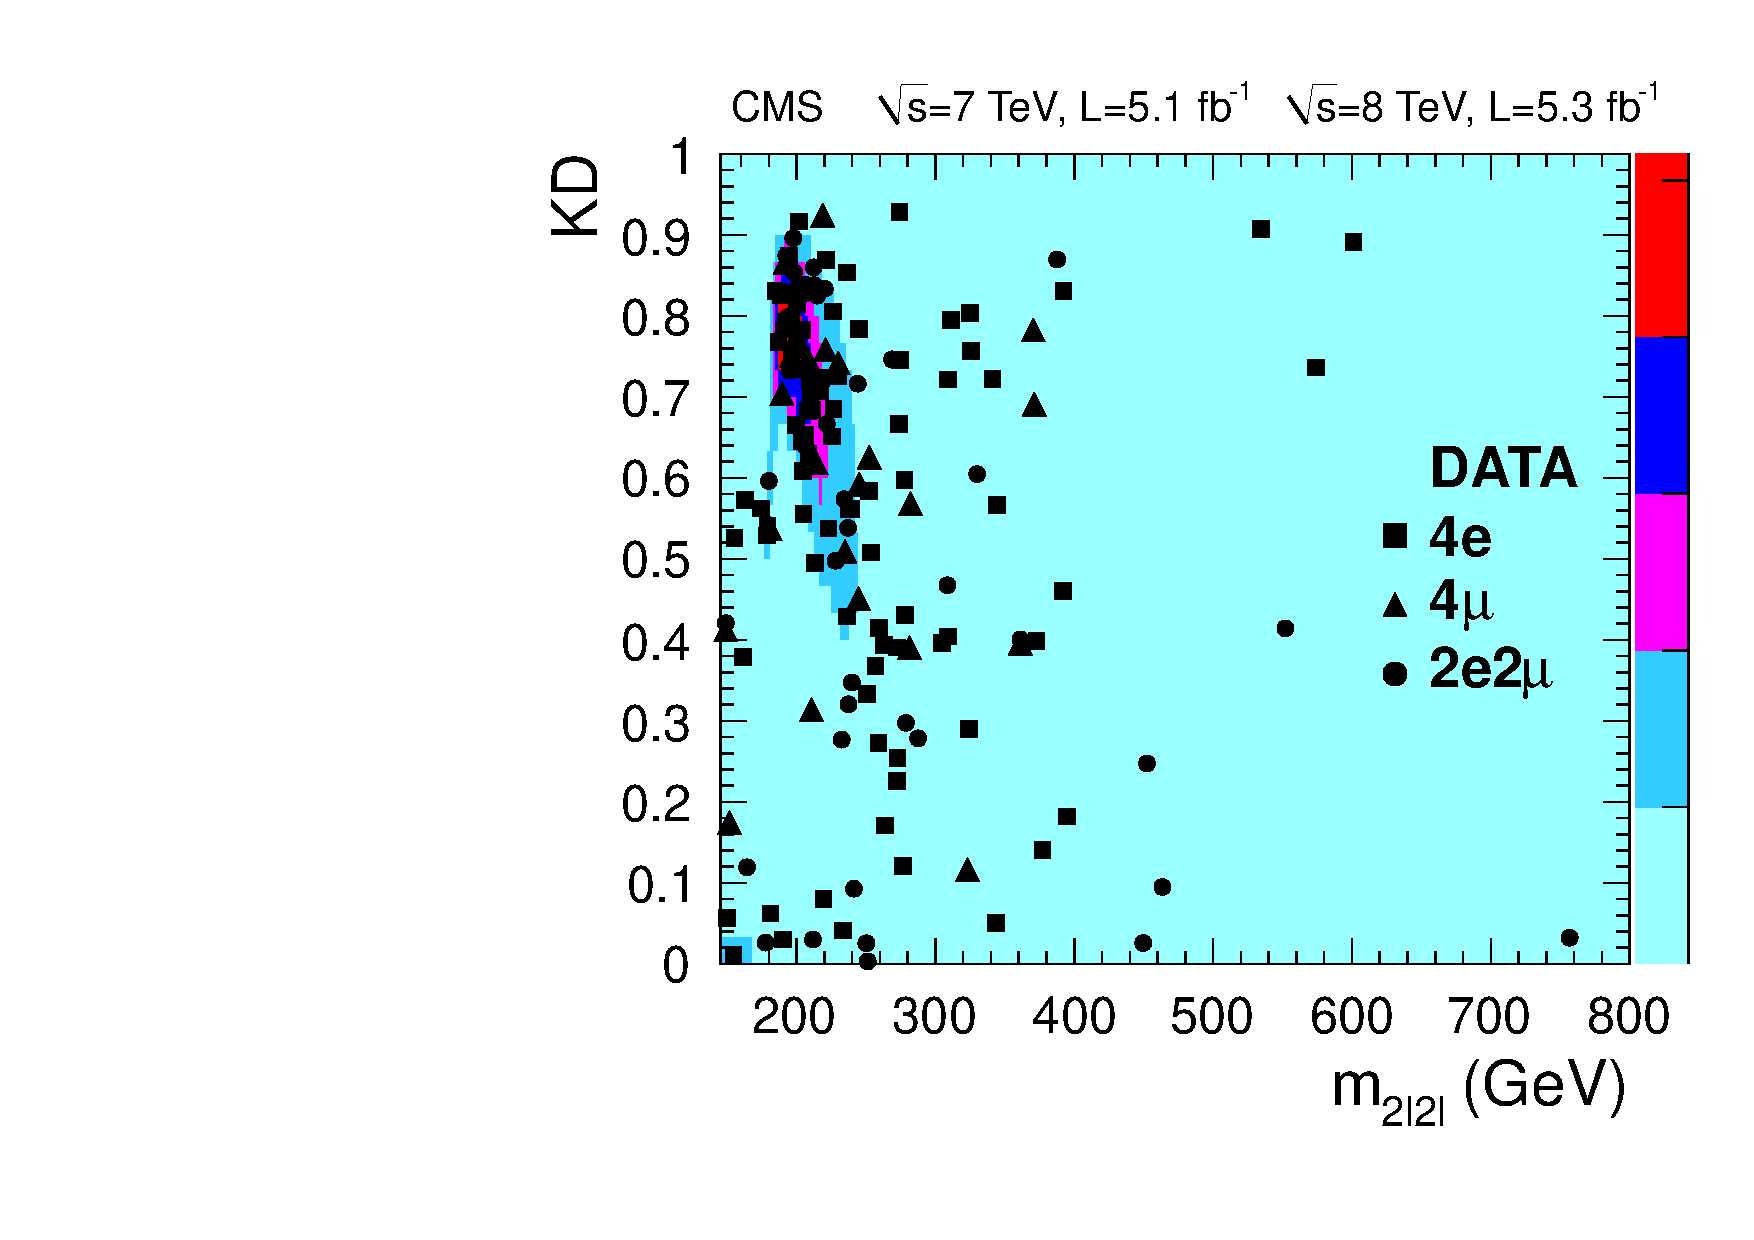
\includegraphics[width=0.45\linewidth]{figures/ZZ4lMELA.pdf}}
\subfigure[]{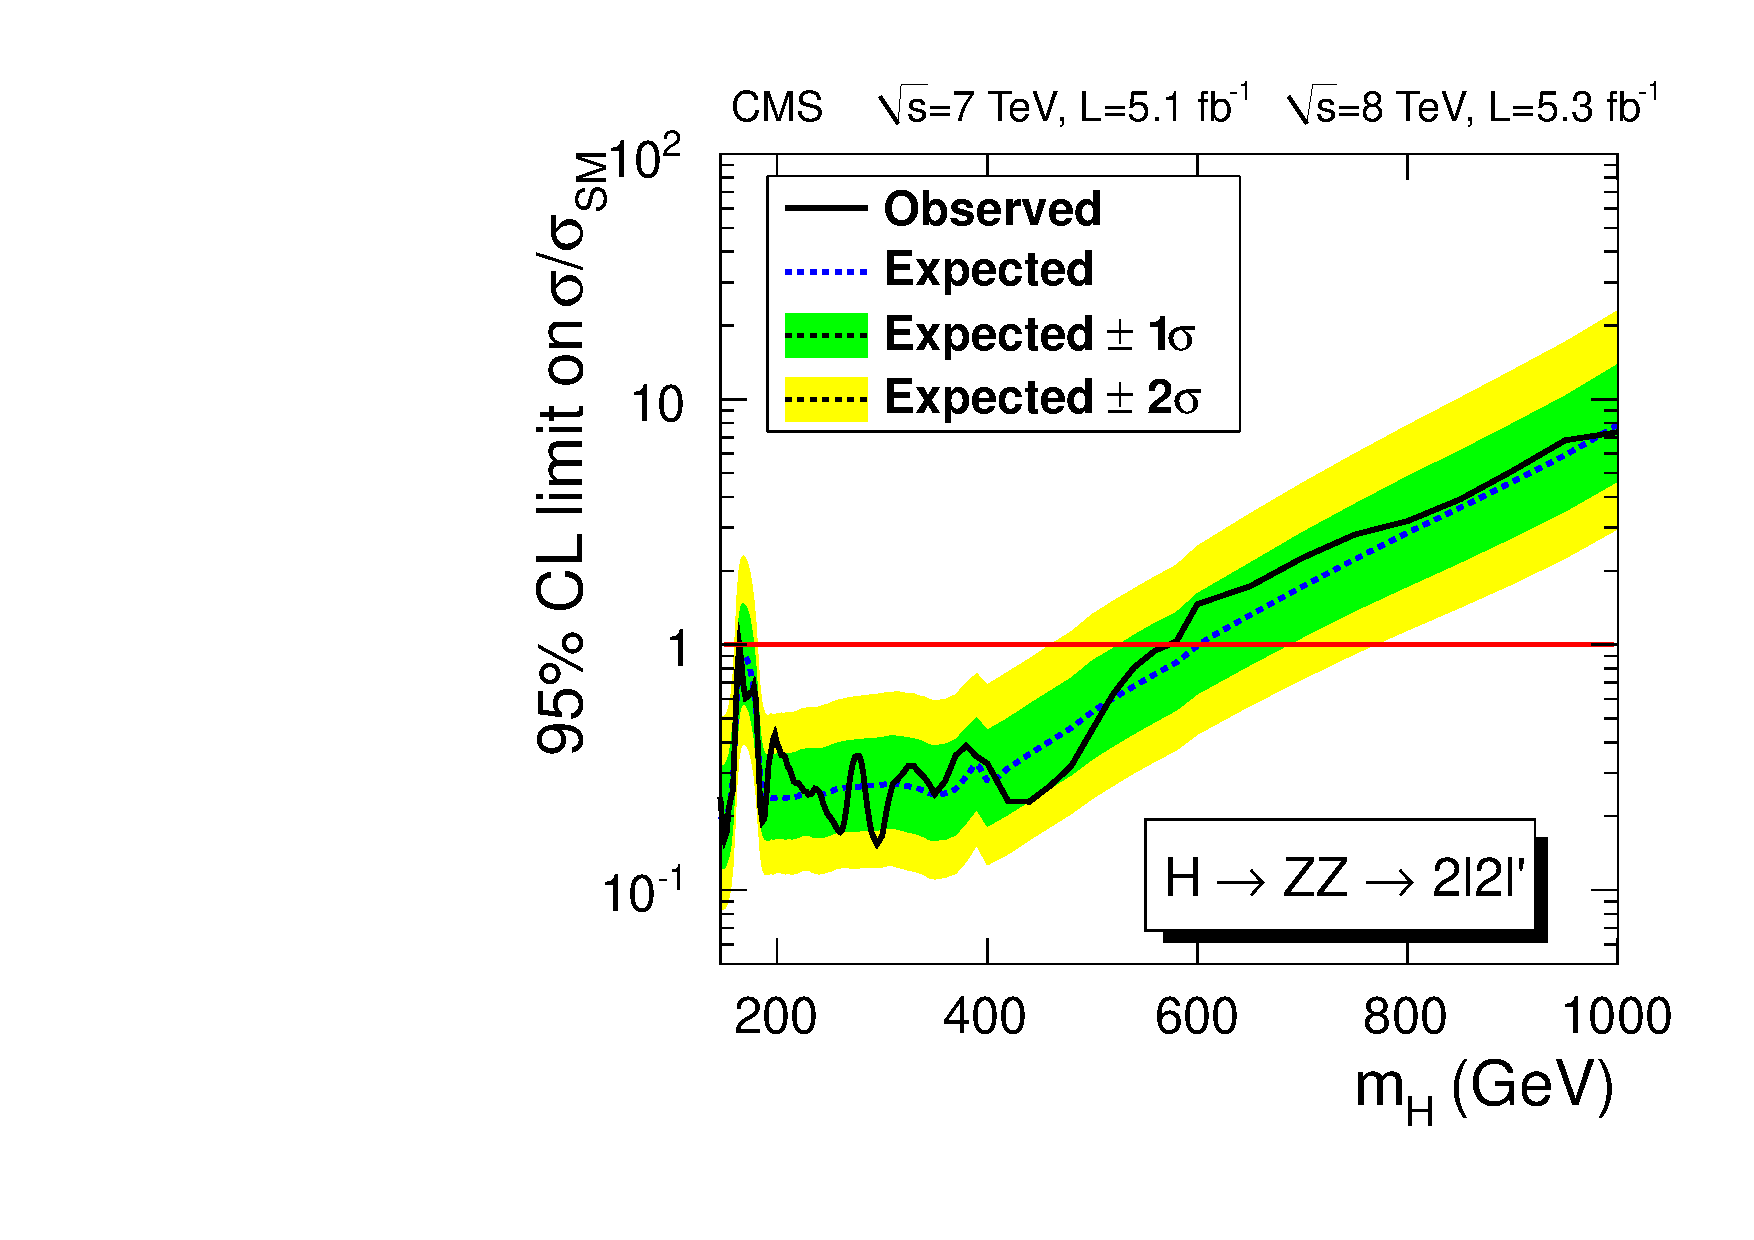
\includegraphics[width=0.45\linewidth]{figures/ZZ4lLimit.pdf}}
%
\caption{ (a) 
The distribution of events
selected in the $2\ell2\ell$ 
subchannels for the kinematic discriminant, KD, versus $m_{2\ell2\ell}$.
Events in the three final states are marked by filled symbols (defined in the legend).
%The horizontal error bars indicate the estimated mass resolution.
The contours represent the expected relative density of background events.
(b) Observed and expected 95\% CL upper limit on the ratio of the product of the production cross section and
 branching ratio to the 
SM expectation in the $\PH \to \ZZ \to 2\ell 2\ell '$ channel.
The 68\% and 95\% ranges of expectation  for the background-only model 
are also shown with green and yellow bands, respectively.
}
\label{fig:KDvsM4lFullMass}
\end{center}
\end{figure}
%=======

The kinematics of the $\PH\to\ZZ \to 2\ell2\ell$ process, for a given invariant mass of the four-lepton system,
are fully described by five angles and the invariant masses of the two lepton pairs~\cite{Cabibbo:1965zz,Gao:2010qx,DeRujula:2010ys}. A kinematic discriminant (KD), based on these seven variables, is constructed based on the probability ratio of the signal and background hypotheses~\cite{2l2qpaper}. The distributions of the $\KD$ versus $m_{2\ell 2\ell}$ is shown in Figure~\ref{fig:KDvsM4lFullMass}(a) for the selected event sample. The distribution of events in the $(m_{2\ell 2\ell}, \KD)$ plane is consistent with the SM background expectation. The
two-dimensional KD-$m_{2\ell2\ell}$ distribution is used to set upper limits on the cross-section in the $2\ell2\ell$ 
channel. For the $2\ell2\tau$ final state, limits are set using the $m_{2\ell2\tau}$ distribution. The combined upper
limits from all channels are shown in Figure.~\ref{fig:KDvsM4lFullMass}(b).

\subsection{$\mathrm{H} \to \ZZ \to 2\ell \mathrm{qq}$}

This channel has the largest branching ratio of all $\mathrm{H} \to \ZZ$ channels, but also a large background
contribution from $\cPZ$+jets production. The hadronically-decaying $\cPZ$ bosons produce quark jets, with a large
fraction of heavy quarks compared to the background that is dominated by gluon and light quark jets. The analysis
presented here updates the previously published result~\cite{2l2qpaper} by the use of the most recent
Higgs lineshape reweighting, amongst other improvements. It also uses only the $\sqrt{s}=7\TeV$ data sample.

Reconstructed decay electrons and muons are required to have $\PT$ greater than 40\GeV and 20\GeV for the leading
and second lepton respectively. Muons are required to have $|\eta|<2.4$, and electrons $|\eta|<2.5$, with the transition
region between ECAL barrel and endcap, $1.44<|\eta|<1.57$, also excluded in the latter case. Jets are required to have
$\PT>30\GeV$ and $|\eta| < 2.4$. Each pair of oppositely-charged leptons of the same flavor, and each pair of jets,
are considered as $\cPZ$ candidates. Background contributions are reduced by requiring $75<\mjj<105\GeV$ and $70<\mll<110\GeV$.

In order to exploit the different jet composition of signal and background, events are classified into three
mutually exclusive categories, according to the number of selected $\cPqb$-tagged jets: 0-b-tag, 1-b-tag and 2-b-tags.
An angular likelihood discriminant is used to separate signal-like from background-like events in each category~\cite{Gao:2010qx}. A 'quark-gluon' likelihood discriminant ($\mathrm{qg}$LD), intended to distinguish gluon
jets from light-quark jets, is employed for the 0-b-tag category, which is expected to be dominated by $\cPZ$+jets
background. In order to suppress the substantial expected $\ttbar$ background in the 2-b-tag category, a discriminant
$\lambda$ is used, defined as the ratio of the likelihoods of a hypothesis with $\MET$ equal to the value measured with
the PF algorithm, and the null hypothesis $\MET=0$~\cite{Chatrchyan:2011tn}. This discriminant provides a measure of
whether the event contains genuine missing transverse energy. Events in the 2-b-tag category are required to
have $2\ln{\lambda} < 10$. When an event contains multiple $\cPZ$ candidates passing the selection requirements,
only the ones with jets in the highest b-tag category are retained for analysis. If multiple candidates are
present, the ones with $\mjj$ and $\mll$ values closest to the $\cPZ$ mass are retained.

The statistical analysis is based on the invariant mass of the Higgs boson candidate, $\mZZ$, which is calculated
using a fit of the final state four momenta, and applying the constraint that the dijet invariant mass is consistent
with the mass of the $\Zo$ boson. Data containing a Higgs boson signal are expected to show a resonance peak in addition
to the continuum background distribution.

%% ED: Does 'consistent' mean 'equal to' here? Or is some range of Z mass taken?

The background distributions are estimated from the  $\mjj$ sidebands, defined as $60<\mjj<75\GeV$ and
$105 <\mjj<130\GeV$. In simulation, the composition and distribution of the dominant backgrounds in the sidebands
are observed to be similar to that in the signal region. The distributions derived from data sidebands are measured
for each of the three b-tag categories and used to estimate the normalization of the background and its dependence on 
$\mZZ$. The results of the sideband interpolation procedure are in good agreement with the observed distributions in
data. In all cases, the dominant backgrounds include $\cPZ$+jets with either light- or heavy-flavor jets and top
background, both of which populate the $\mjj$ signal region and the $\mjj$ sidebands. The diboson background amounts
to less than 5\% of the total in the 0- and 1-b-tag categories, and about 10\% in the 2-b-tag category. No significant 
difference is observed between results from data and the background expectation. The expected and observed event yields
are listed in Table~\ref{table-yields}.

%%%%%%%%%%%%%%%%%%%%%%%%%%%%%%%%%%%%%%%%%%%%%%%%%
\begin{table}[htbp]
\begin{center}
\caption{
Observed and expected event yields in the $\mathrm{H} \to \ZZ \to 2\ell \mathrm{q\bar{q}}$ channel
The expected background is quoted from the $\mjj$ sideband procedure and from simulation (MC).
The uncertainties are statistical only.}
\label{table-yields}
\begin{tabular}{l|c|c|c}
\hline
Category & 0 \cPqb-tag & 1 \cPqb-tag &  2 \cPqb-tag \\
\hline
Background ($\mjj$ sideband)   & $3041\pm54$  & $3470\pm59$  & $258\pm17$  \\
Background (MC)     & $3105\pm39$  & $3420\pm41$  & $255\pm11$  \\
\hline
Observed  & 3036         & 3454         & 285\\
\hline
\mH=550\GeV        &  6.5 $\pm$ 1.0  & 6.5  $\pm$ 0.9  & 3.6  $\pm$ 0.8 \\
\hline
\end{tabular}
\end{center}
\end{table}

%%%%%%%%%%%%%%%%%%%%%%%%%%%%%%%%%%%%%%%%%%%%%%%%%
%\begin{widetext}
%%%%%%%%%%%%
%\begin{figure}[htbp]
%\begin{center}
%\subfigure[]{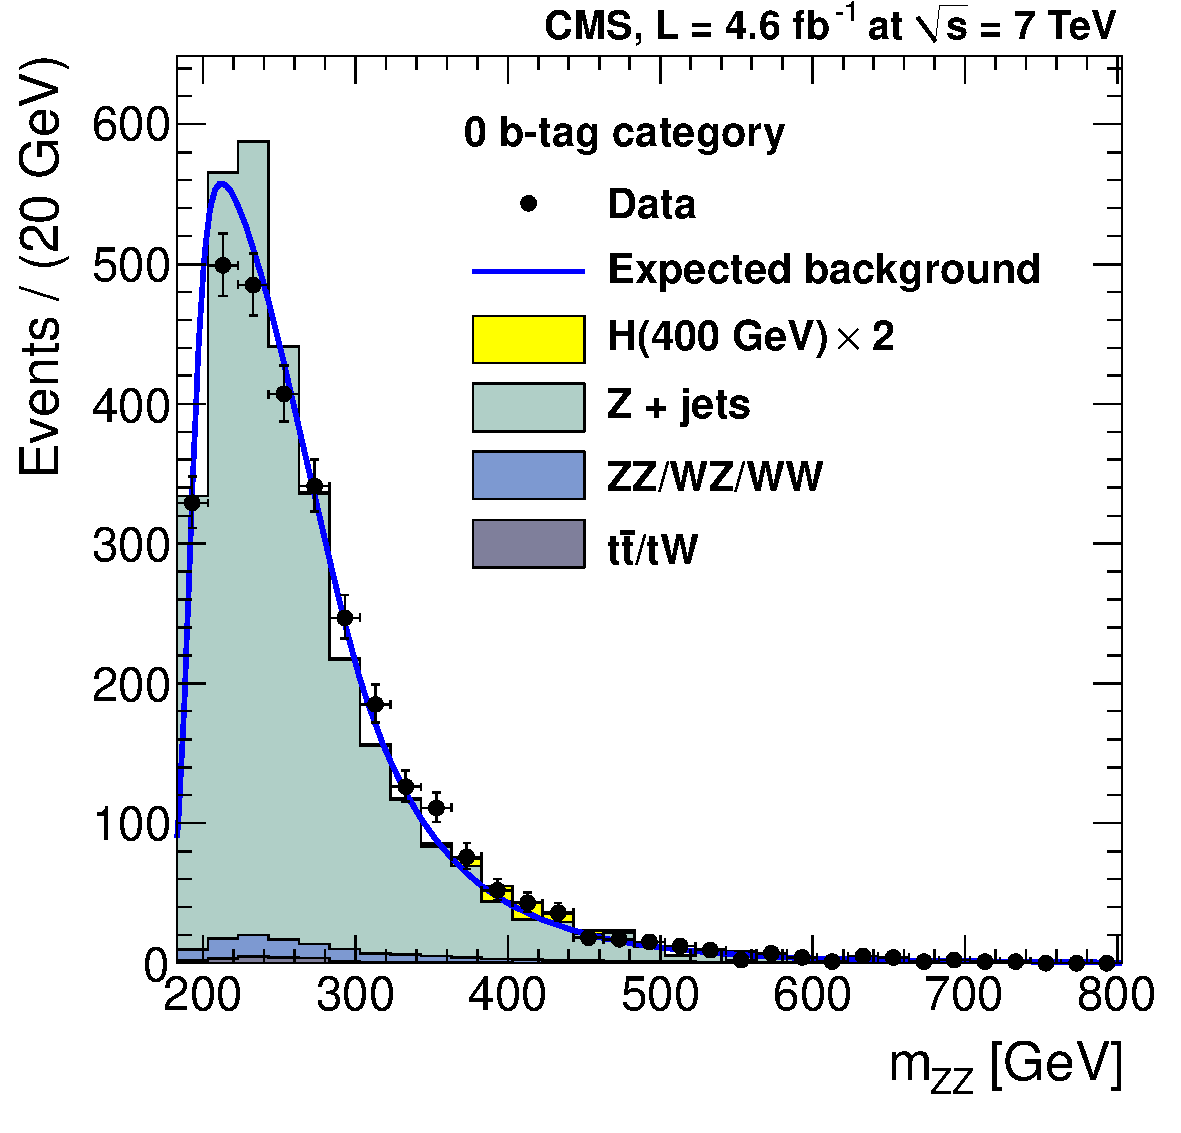
\includegraphics[width=0.3\textwidth]{plots/mzz_0btag.pdf}}
%\subfigure[]{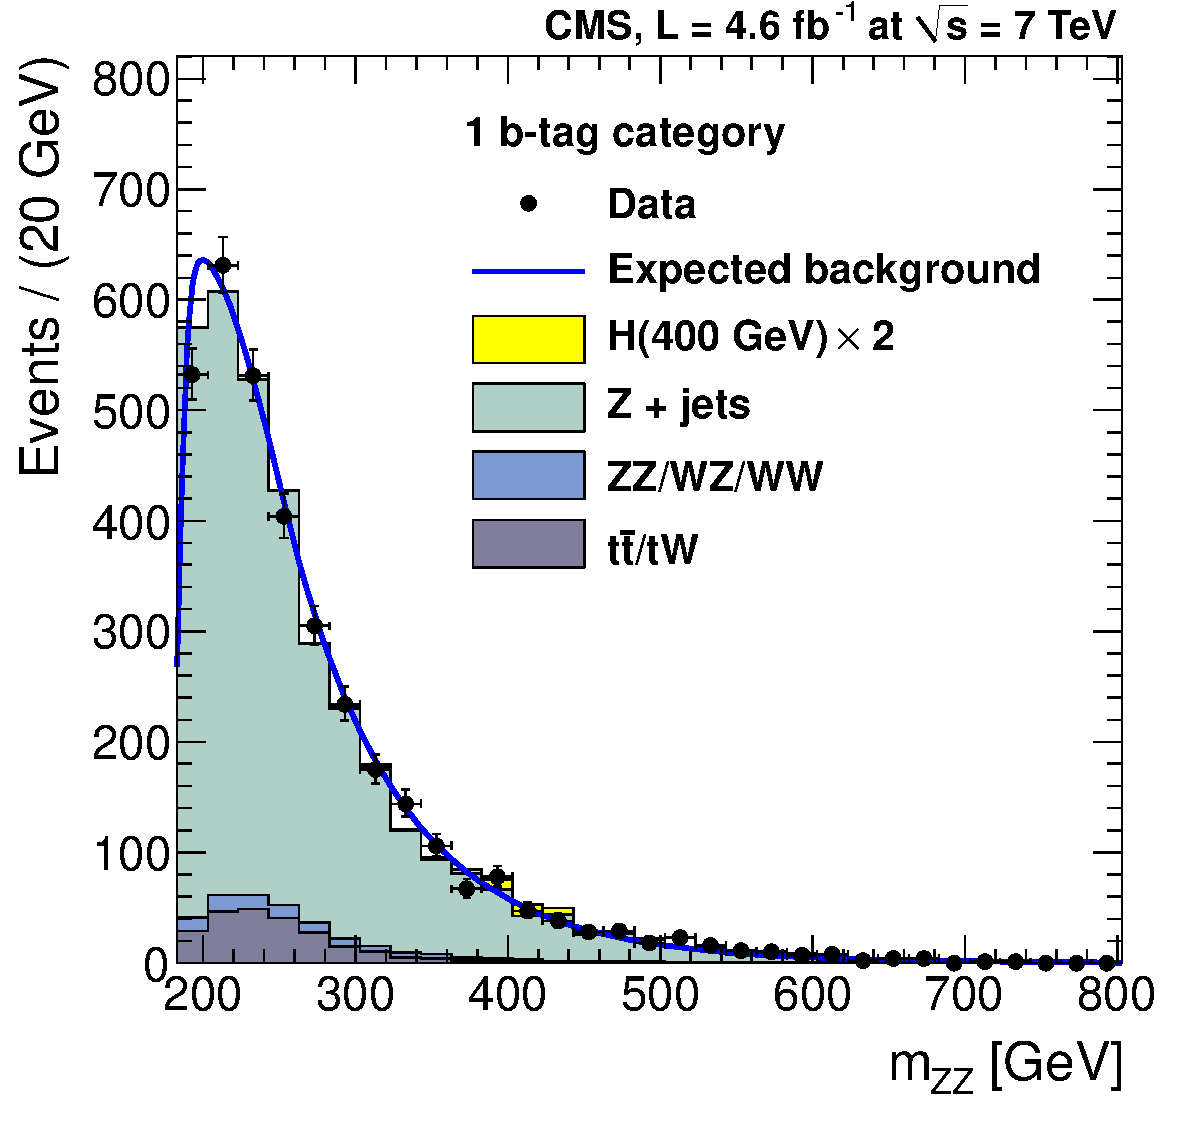
\includegraphics[width=0.3\textwidth]{plots/mzz_1btag.pdf}}
%\subfigure[]{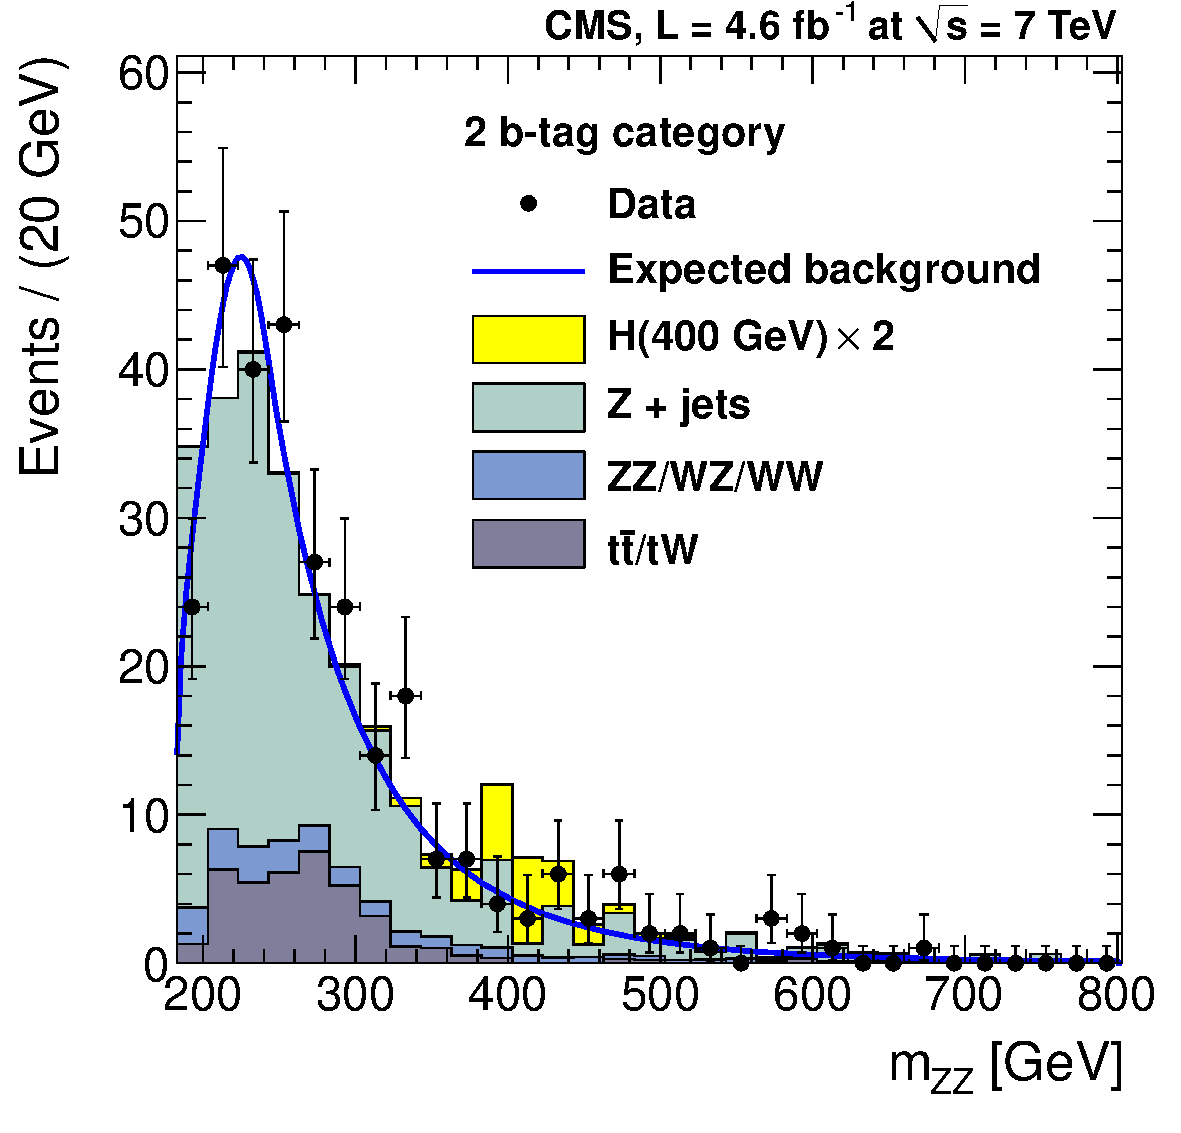
\includegraphics[width=0.3\textwidth]{plots/mzz_2btag.pdf}}
%\caption{
%The $\mZZ$ invariant mass distribution after final selection in three categories:
%(a) 0~\cPqb-tag,
%(b) 1~\cPqb-tag, and
%(c) 2~\cPqb-tag.
%Points with error bars show distributions of data and
%solid curved lines show the prediction of background from the sideband extrapolation procedure.
%In the low-mass range, the background is estimated from the $\mZZ$ sideband for each Higgs
%mass hypothesis and the average expectation is shown.
%Solid histograms depicting the background expectation from
%simulated events for the different components are shown.
%Also shown is the SM Higgs boson signal with the mass of 400\GeV and cross section
%2 times that of the SM Higgs boson, which roughly corresponds to expected exclusion
%limits in each category.
%}
%\label{fig:mZZ_kinfit_hiMass}
%\end{center}
%\end{figure}

\begin{figure}[htbp]
\begin{center}
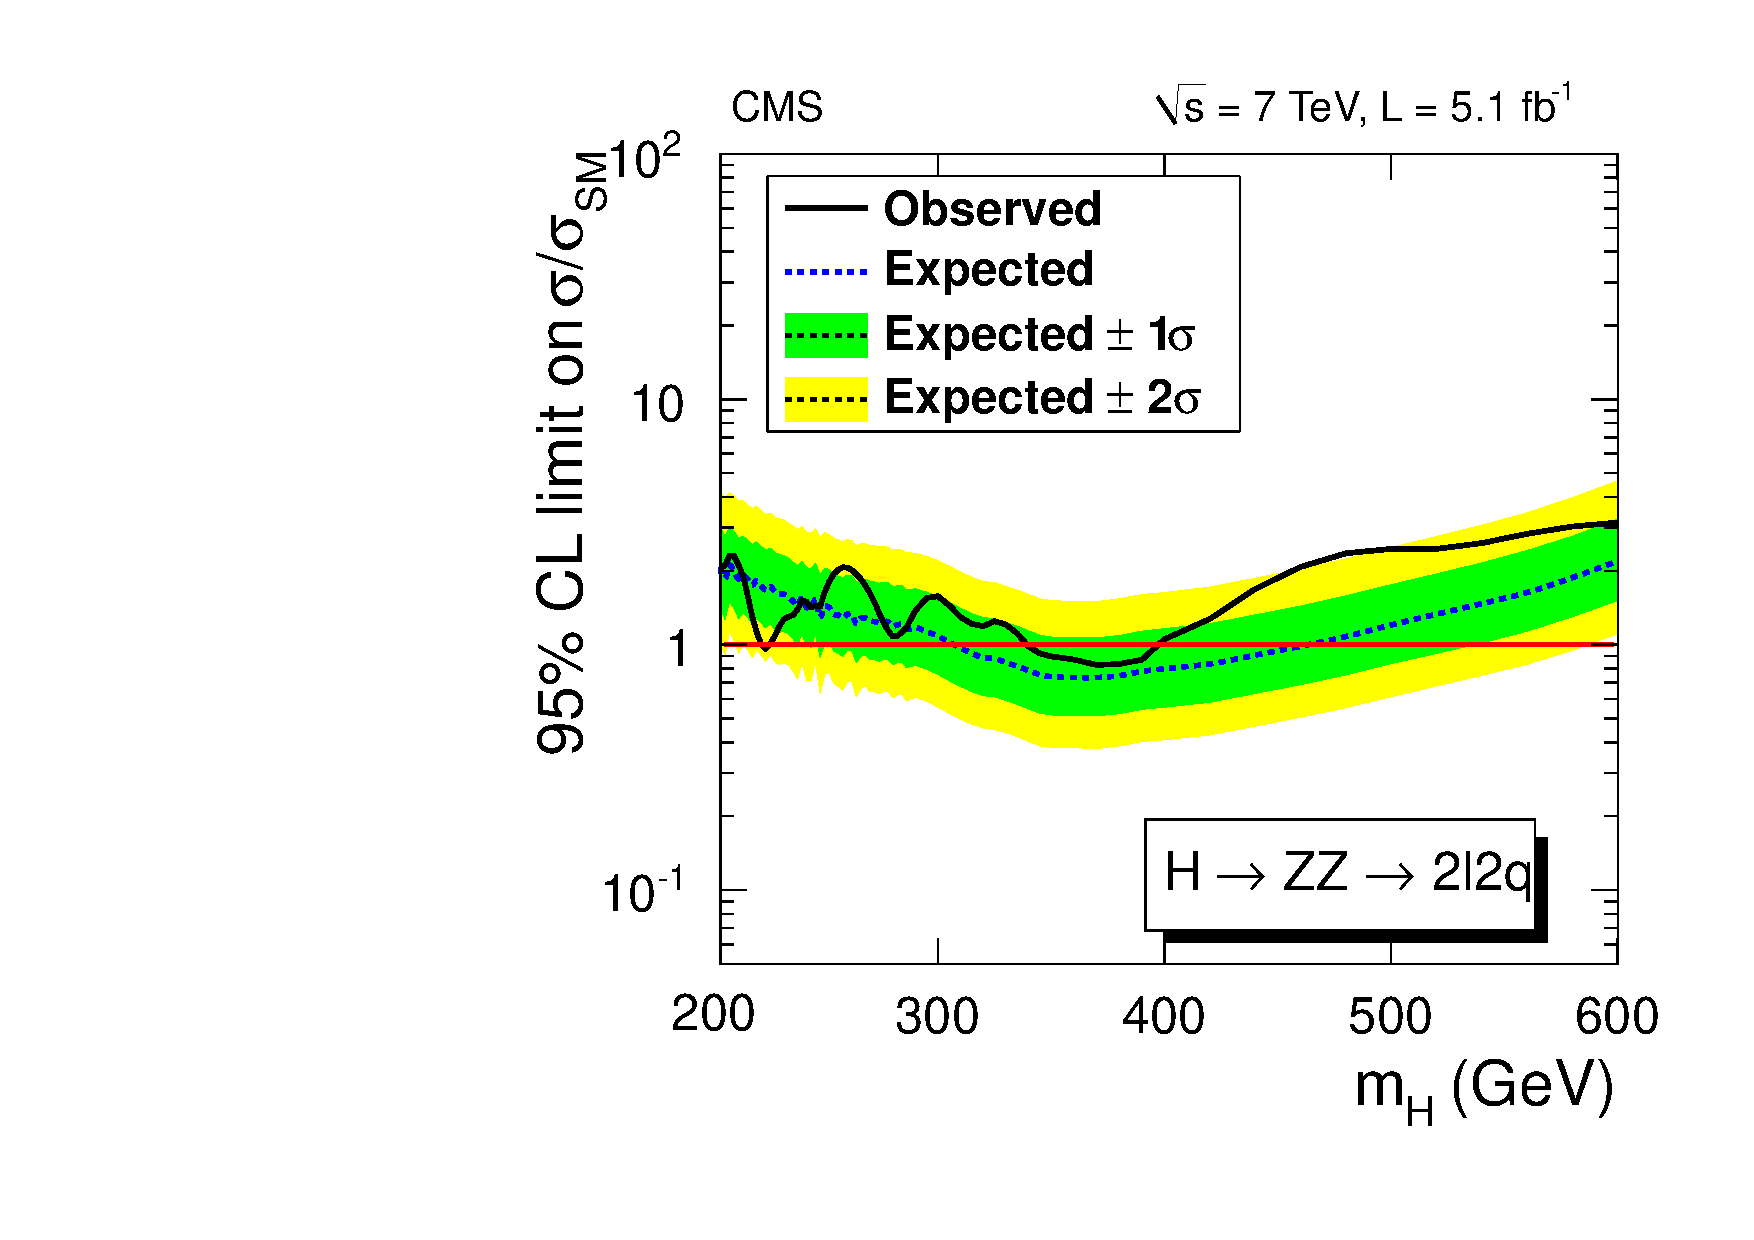
\includegraphics[width=0.6\linewidth]{figures/ZZ2l2qLimit.pdf}
\caption{
Observed (solid) and expected (dashed) 95\% CL upper limit on the ratio of the product of the production cross section
and branching ratio, to the SM expectation for the Higgs boson in the $\mathrm{H} \to \ZZ \to 2\ell \mathrm{q\bar{q}}$ channel.
}
\label{fig:ZZ2l2qlimit}
\end{center}
\end{figure}

The distribution of $\mZZ$ for the background is parameterized with an empirical function, fitted to the shape and normalization determined from the sidebands. The dominant normalization uncertainty in the background estimation
is due to statistical uncertainty of the number of events in the sidebands. The reconstructed signal distributions are 
described with a Gaussian function with power-law tails, and an empirical function representing the misreconstruction of
the Higgs boson decay products. The signal reconstruction efficiency and the $\mZZ$ distribution are parameterized as a 
function of $\mH$, and are extrapolated to all mass points. The main uncertainties in the signal $\mZZ$ parameterization
are due to experimental resolution, which is predominantly due to the uncertainty on the jet energy scale~\cite{Chatrchyan:2011ds}. Uncertainties due to b-tagging are evaluated with a sample of jet events enriched in
heavy flavors by requiring a muon to be spatially close to a jet. The uncertainty associated with the $\mathrm{qg}$LD 
selection efficiency is evaluated using the $\Pgg+\text{jet}$ sample in data, which predominantly contains quark jets.

The upper limits at 95\% CL, on the ratio of the production cross section for the Higgs boson to the SM expectation,
obtained from the combination of all categories, are presented in Figure~\ref{fig:ZZ2l2qlimit}.
This exclusion limit supersedes the previously published one~\cite{2l2qpaper} as a result of
an improved signal lineshape description and the correction of
a problem
in the background
description. The latter resulted in an overly conservative estimate of expected sensitivity in
the previous analysis~\cite{2l2qpaper}.

\subsection{$\PH \to \ZZ \to 2\ell 2\nu$}

This analysis identifies Higgs boson decays to a pair of $\cPZ$ bosons, with one $\cPZ$ decaying to neutrinos. The
analysis strategy is based on selection requirements in the (\MET,\MT) phase space, with selections adjusted for
different $\mH$ hypotheses. A detailed description of the analysis can be found in~\cite{Chatrchyan:2012ft}.

Events are required to have a pair of well-identified, isolated leptons of same flavour ($\Pep\Pem$ or $\Pgmp\Pgmm$),
each with $\PT > 20\GeV$, with an invariant mass within a $30\GeV$ window centered on the $\cPZ$ mass. The $\PT$
of the dilepton system is required to be greater than $55\GeV$. The presence of large missing transverse energy in the
event is also a fundamental feature of the signal.

To suppress $\cPZ$+jets background, events are removed from the analysis if the angle in the azimuthal plane between
the \MET and the closest jet with transverse energy $\ET > 30\GeV$ is smaller than 0.5 radians. In order to remove events where the lepton is mismeasured, events are rejected if \MET$>$60\GeV and $\Delta\phi$($\ell$,\MET)$<0.2$. The top quark background is suppressed by applying a veto on events having a b-tagged jet with $\ET > 30\GeV$ and $|\eta| < 2.5$.
To further suppress the top-quark background, a veto is applied on events containing a 'soft muon', with $\PT > 3\GeV$, which is typically produced in the leptonic decay of a b quark. To reduce the $\PW\cPZ$ background, in which both bosons
decay leptonically, any event with a third lepton ($\Pe$ or $\Pgm$) with $\PT > 10\GeV$, and passing the identification and
isolation requirements, is rejected.

The search is carried out in two mutually-exclusive categories. The VBF category contains events with two or more jets
in the forward region, with a $|\Delta\eta|>4$ between the two closest jets, and with the invariant mass of those two
jets greater than $500\GeV$. In addition, the two leptons forming the $\cPZ$ candidate are required to lie in between
these two jets, while no other selected jets are allowed in this central region. The gluon fusion category includes all events failing the VBF selection, and is subdivided into subsamples according to the presence or absence of
reconstructed jets with $\PT>$30~\GeV. The event categories are chosen in order to optimize the expected cross-section
limit. In the case of the VBF category, a constant $\MET>70\GeV$ and no $m_\mathrm{T}^{\ell\ell,\MET}$ requirement are used as no gain in sensitivity is obtained with a Higgs-mass-dependent selection.

%% ED: As opposed to what? What is done in the other categories? Looks like it was in the table which has now been excluded, so this needs to be fixed.

%% ED: What does 'selected jets' mean here?

%\begin{table}[htbp]
%\caption{
%      Higgs boson mass-dependent selection for \MET and
%      $\MT$ variables in the 
%      %and shape-based 
%      gluon fusion analysis.}
%\begin{center}
%\begin{tabular}{c|ccccc}\hline
%$\mH$ (\GeVns)    & 200        & 300        & 400         & 500        & $\geq$600 \\
%\hline
%\hline
%\MET (\GeVns)     & $>75$     & $>85$     & $>90$      & $>90$     & $>100$  \\
%$M_T$ (\GeVns)    & $175 - 275$ & $250 - 375$ & $325 - 450$  & $400 - 650$ & $450 - \infty$ \\
%\hline
%\end{tabular}
%\end{center}
%\label{tab:met_mtcuts}
%\end{table}

The background composition is expected to vary with the hypothesised value of $\mH$. At low $\mH$, $\cPZ$+jets
and $\ttbar$ are the largest contributions, whilst at higher $\mH$ (above 400 GeV), the irreducible $\cPZ\cPZ$ and
$\PW\cPZ$ backgrounds dominate. The $\cPZ\cPZ$ and $\PW\cPZ$ backgrounds are taken from simulation and are
normalized to their respective NLO cross sections. The $\cPZ$+jets background is modeled from an orthogonal control
sample of events with a single photon produced in association with jets. This procedure yields an accurate model of
the \MET distribution in $\cPZ$+jets events, shown in Figure~\ref{fig:zgamma_met_data}.

\begin{figure}[htbp]
\begin{center}
\subfigure[]{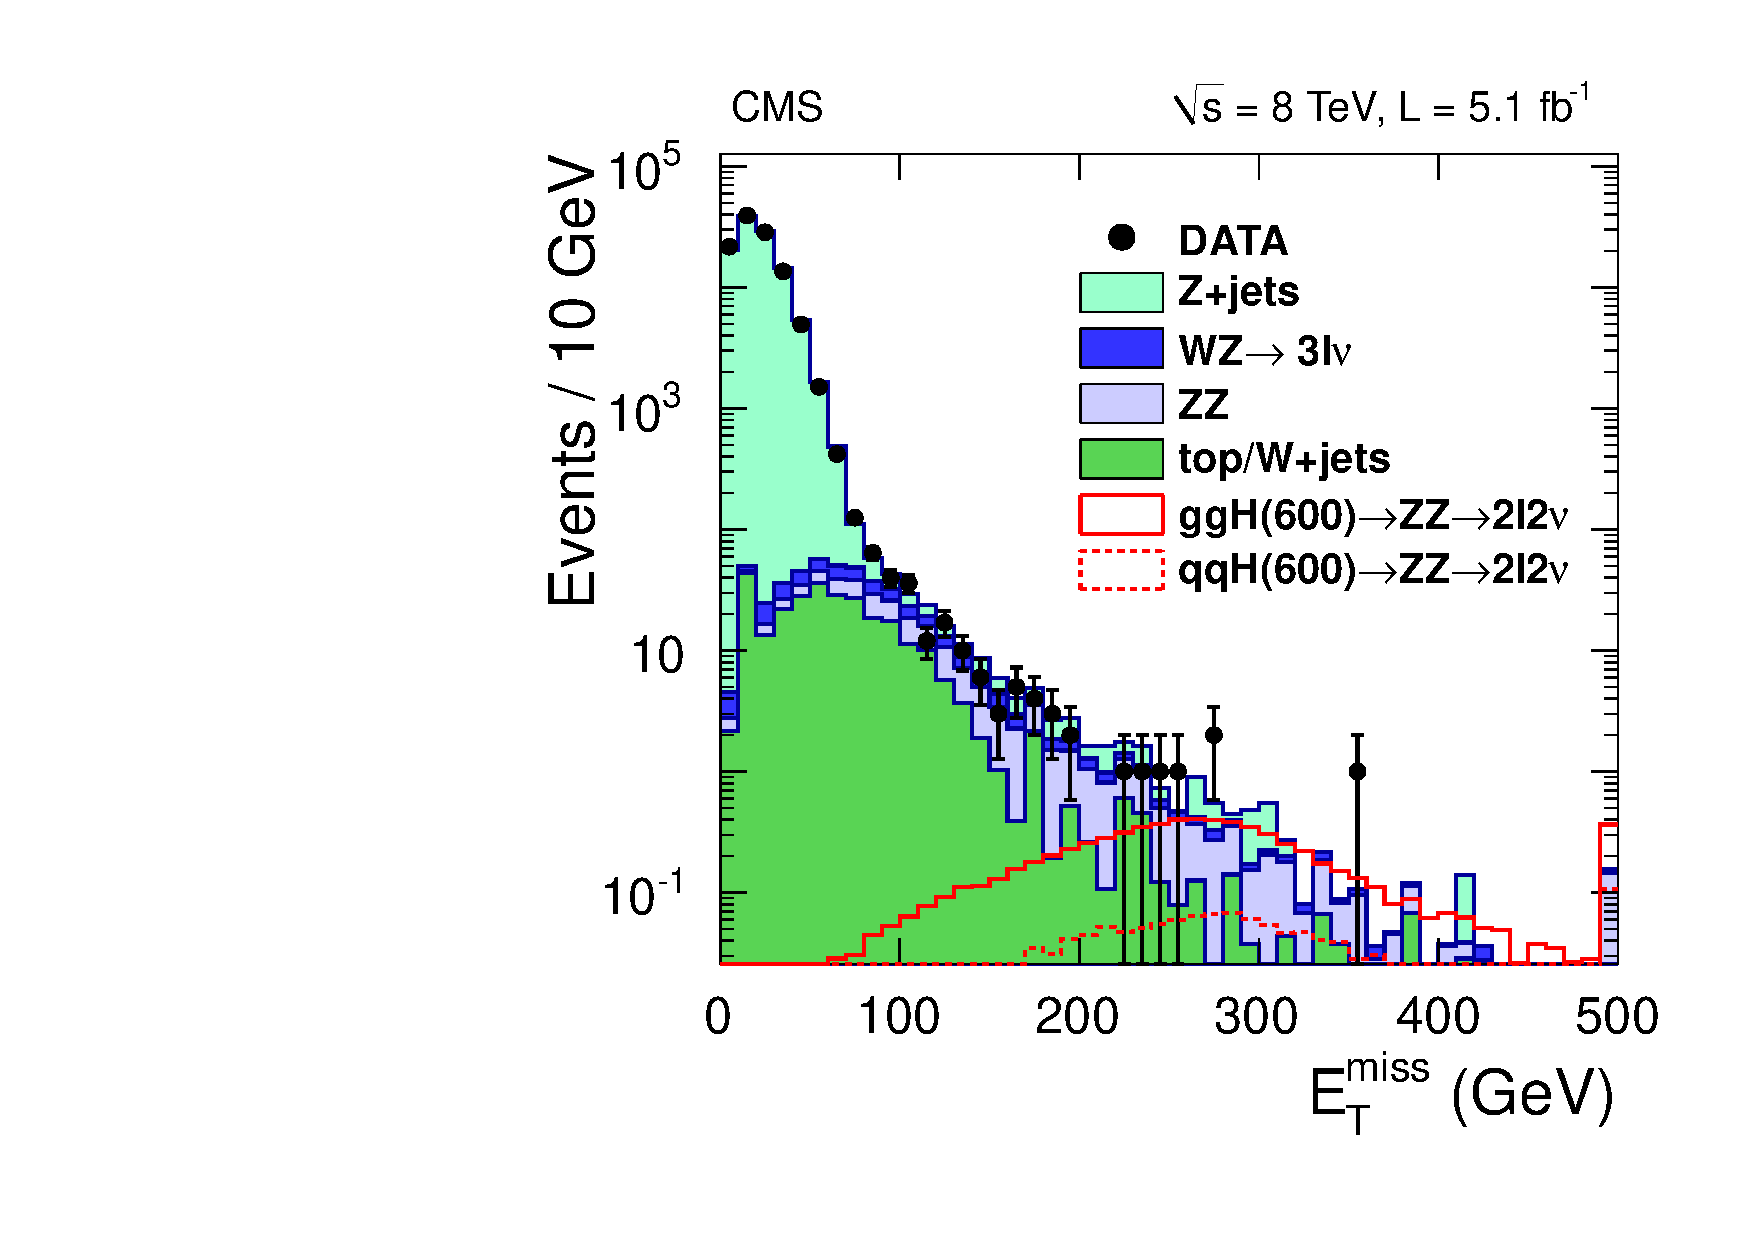
\includegraphics[width=0.45\textwidth]{figures/ZZ2l2nuNoVBF.pdf}}
\subfigure[]{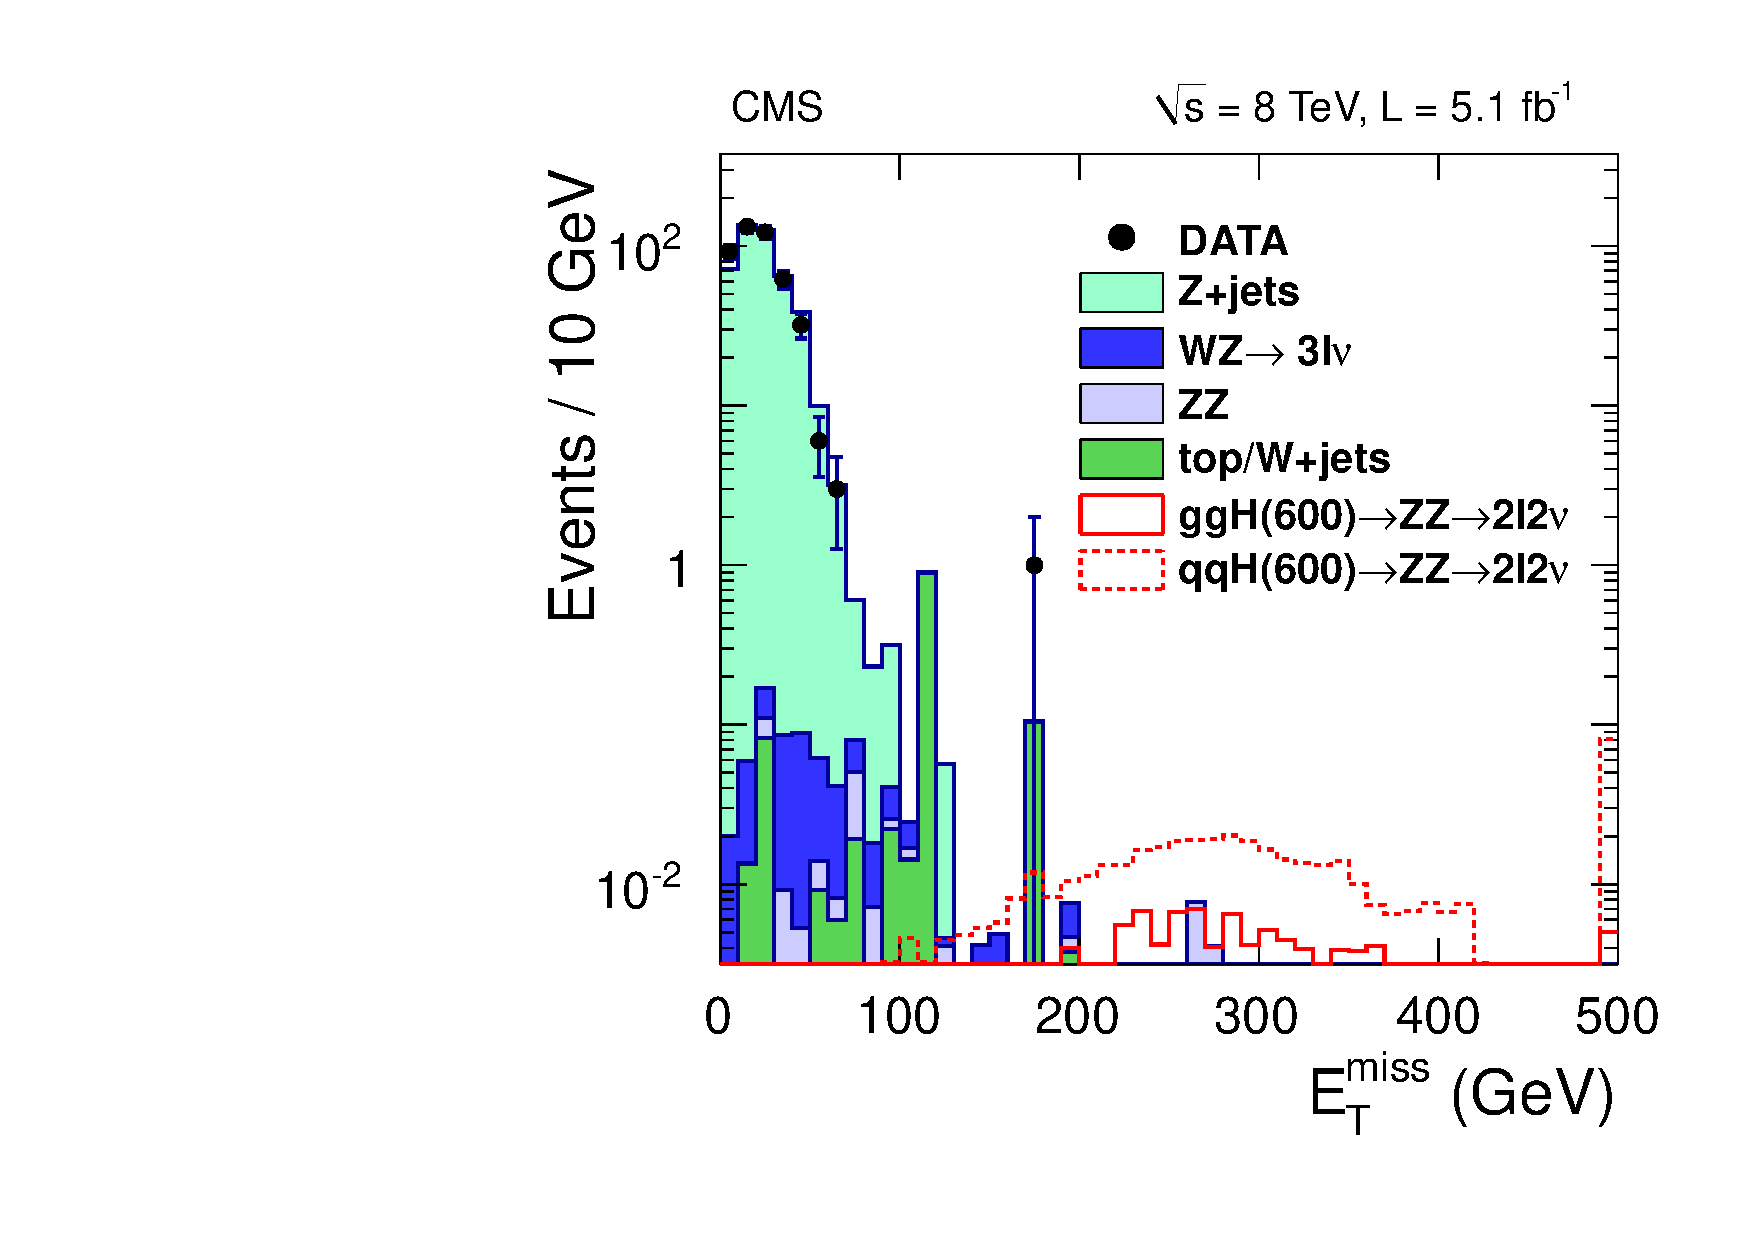
\includegraphics[width=0.45\textwidth]{figures/ZZ2l2nuVBF.pdf}}
\caption{The \MET distribution in data compared to the estimated background
in the (a) gluon fusion and (b) VBF categories {of the $\PH \to \ZZ \to 2\ell 2\nu$ channel}. 
The dielectron and dimuon channels are combined.
Contributions from $\ZZ$, $\PW\cPZ$, non-resonant background and $\cPZ$+jets background are stacked
on top of each other. The \MET distribution in signal events for $\mH = 600$\GeV is also shown.} 
\label{fig:zgamma_met_data}
\end{center}
\end{figure}

The uncertainty associated with the $\cPZ$+jets background is affected by any residual contamination of the
$\Pgg$+jets control sample from processes involving a photon and genuine $\MET$. We do not explicitly subtract this
contamination, but estimate this background to be 50\% of the background estimate and assign a 100\% uncertainty to it, effectively allowing the limit fit to determine the most likely amount. 

Background processes that do not involve a $\cPZ$ resonance (non-resonant background) are estimated with a control
sample of events with dileptons of different flavor ($\Pe^{\pm}\Pgm^{\mp}$) that pass the full analysis selection.
This method cannot distinguish between the non-resonant background and a possible contribution from
$\PH \rightarrow \PW\PW \rightarrow 2\ell 2\cPgn$ events, which are treated as part of the non-resonant background
estimate. The non-resonant background in the $\Pep\Pem$ and $\Pgmp\Pgmm$ final states is estimated by applying a
scale factor to the selected $\Pe^{\pm}\Pgm^{\mp}$ events, estimated from the sidebands of the $\cPZ$ peak events
($40 < m_{\ell\ell} < 70\GeV$ and $110 < m_{\ell\ell} < 200\GeV$). The uncertainty associated with the estimate of the
non-resonant background is determined to be 25\%. The expected signal and background, and the observed event yields, for 
a $\mH=400\GeV$ hypothesis are listed in Table~\ref{tab:final_yields}. No significant excess of events is observed over
the SM background expectation.

%============
\begin{table}[htbp]
\begin{center}
\caption{
The number of event candidates observed, compared to the mean expected 
background and signal yields for each category {in the $\PH \to \ZZ \to 2\ell 2\nu$ channel}
for the $\mH=400\GeV$ hypothesis with selection requirements $\MET>90\GeV$, $325<\MT<450\GeV$. 
}
\label{tab:final_yields}
\begin{tabular}{l|c|c|c}
\hline
Category & VBF & 0jets & $\geq$1 jets \\
\hline
Background &  3.0 $\pm$ 0.9 $\pm$ 0.4 &  13.8 $\pm$ 0.6 $\pm$ 1.4  &  20.6 $\pm$ 0.9 $\pm$ 3.1 \\ %
\hline
Observed  & 2 & 13  & 24 \\ %
\hline
$\mH = 400\GeV$ & 2.0 $\pm$ 0.1 & 17.2 $\pm$ 0.1 & 22.1 $\pm$ 0.1 \\ % 
\hline
\end{tabular}
\end{center}
\end{table}

The observed and expected upper limits as a function of $\mH$ are shown in Figure~\ref{fig:limits_SM}. 
%The SM Higgs
%boson is excluded in the mass range 220 to 675\GeV at 95\% confidence level, compared to an expected exclusion range of 275 to 630\GeV.

\begin{figure}[htbp]
\begin{center}
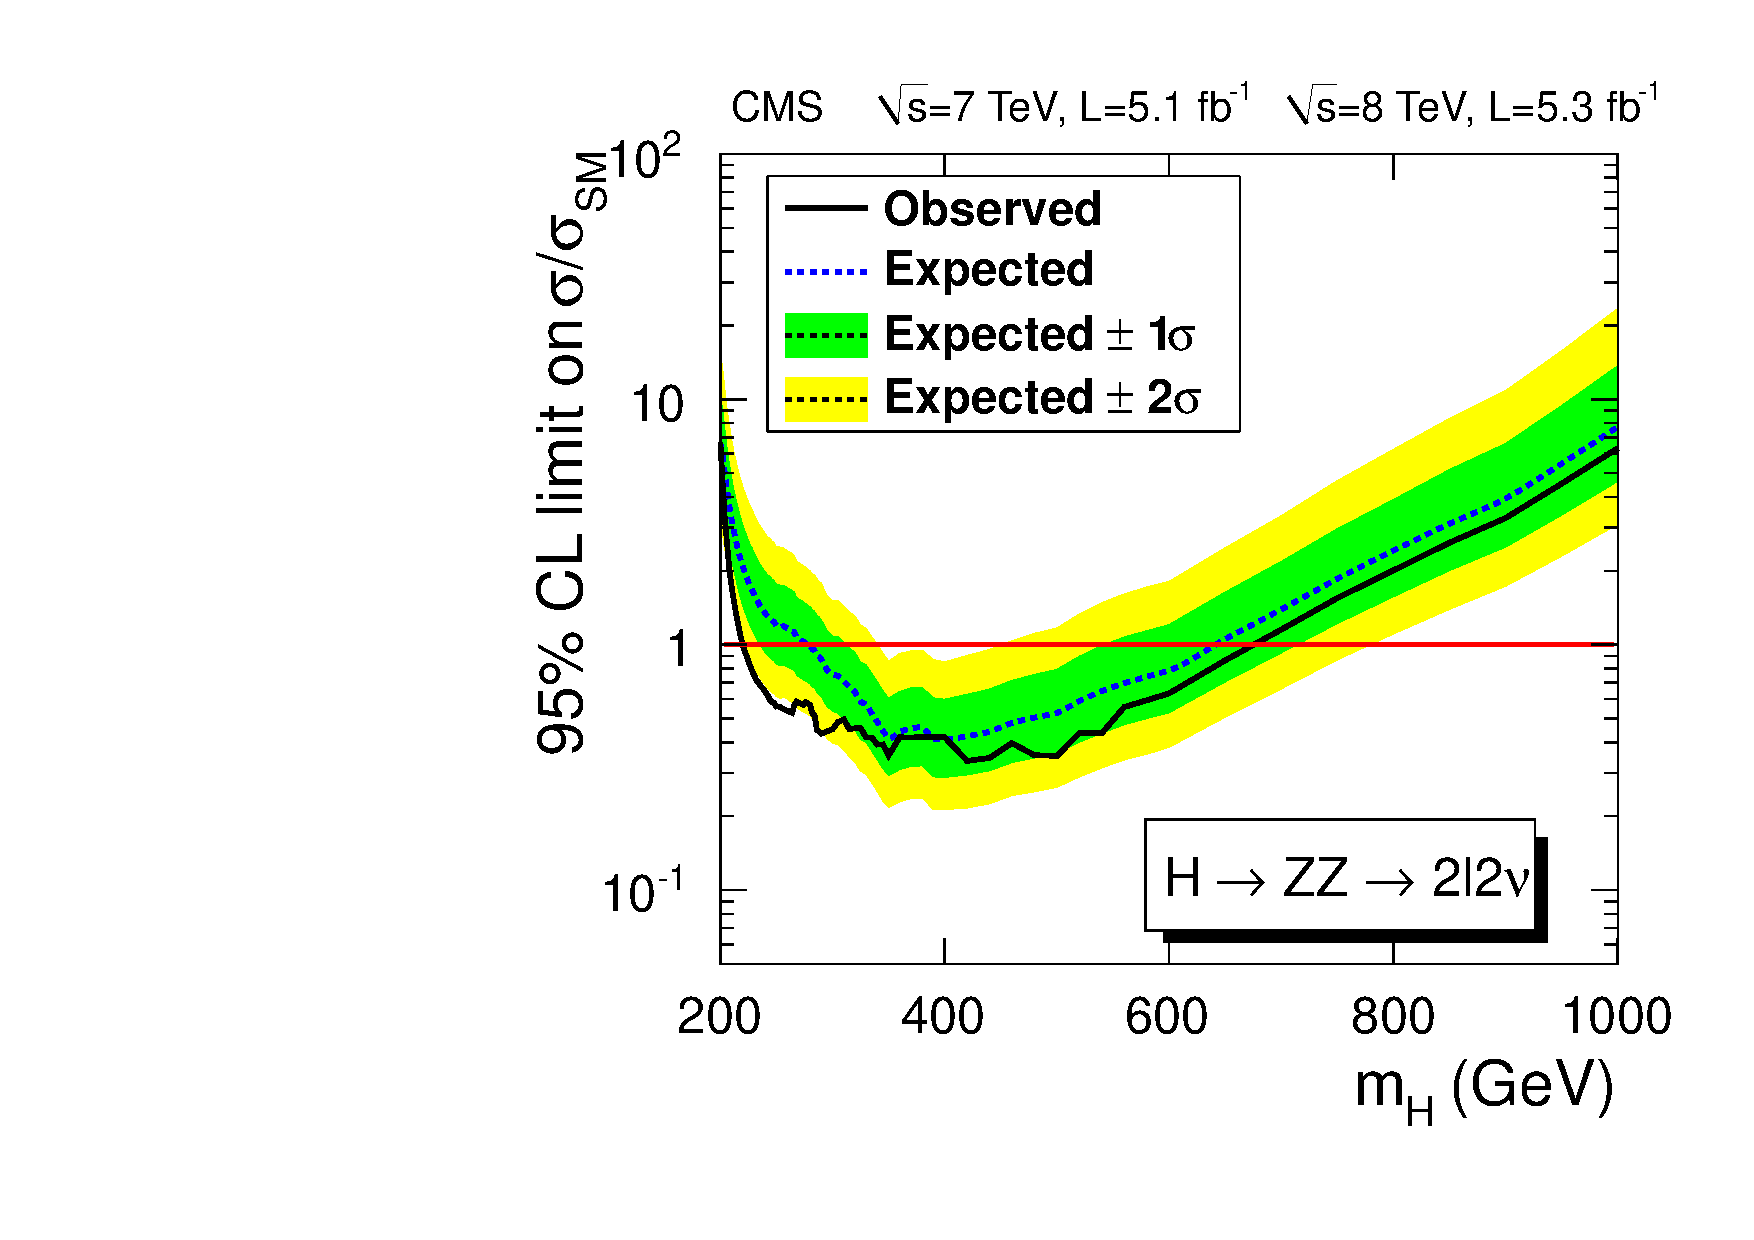
\includegraphics[width=0.6\textwidth]{figures/ZZ2l2nuLimit.pdf}
\caption{Observed (solid) and expected
(dashed) 95\% CL upper limit on the ratio of the product of the  production cross
section and branching ratio to the SM expectation for the Higgs boson for the $\PH \to \ZZ \to 2\ell 2\nu$ channel.
} 
\label{fig:limits_SM}
\end{center}
\end{figure}
